% Template for SSP-2016 paper; to be used with:
%          spconf.sty  - ICASSP/ICIP LaTeX style file, and
%          IEEEbib.bst - IEEE bibliography style file.
% --------------------------------------------------------------------------
\documentclass{article}
\usepackage{spconf,amsmath,epsfig}
\usepackage{amssymb}
\usepackage{amsthm}
\usepackage{algorithm}
\usepackage{algpseudocode}
%\usepackage{fullpage}
\usepackage{tikz}
\usepackage{graphicx}
\usepackage{subfig}
\usepackage{epstopdf}
\usepackage{epsfig}
\usetikzlibrary{tikzmark,calc}
\usepackage{caption}
\usepackage{float}
\usepackage{multirow}
\usepackage{todonotes}
\usepackage{microtype}
\usepackage{hyperref}
\usepackage{mathtools}
\usepackage{pgfplots}
\usepackage{rotating}
\numberwithin{equation}{section} 
\newtheorem{theorem}{Theorem}[section]                   %[section]   %numberes automatically
\newtheorem{lemma}[theorem]{Lemma}         %[theorem]  in the middle
\newtheorem{corollary}[theorem]{Corollary}     %{corollary}{Corollary}[theorem]   
\newtheorem{proposition}[theorem]{Proposition}
\newtheorem{claim}[theorem]{Claim}
\newtheorem{ass}[theorem]{Assumption}
\newtheorem{fact}[theorem]{Fact}
\newtheorem{heuristic}[theorem]{Heuristic}
\newtheorem{definition}[theorem]{Definition}
\newtheorem{remark}[theorem]{Remark}
\newtheorem{exmp}[theorem]{Example} 
\newcommand{\SREC}{S-REC}
\DeclareMathOperator*{\argmin}{arg\,min}
\DeclareMathOperator*{\argmax}{arg\,max}
\def\R{{\mathbb{R}}}

\def\sgn{\mathrm{sgn}}
\def\card{\mathrm{card}}
\def\t{\intercal}
\def\t{\top}
\def\cosamp{\mathrm{CoSaMP}}
\newcommand{\mb}[1]{\mathbf{#1}}
\DeclarePairedDelimiter{\diagfences}{(}{)}
\newcommand{\diag}{\operatorname{diag}\diagfences}

\newcommand{\eps}{\epsilon}
\newcommand{\wh}[1]{\widehat{#1}}
\newcommand{\s}{0.18}

% Example definitions.
% --------------------
\def\x{{\mathbf x}}
\def\L{{\cal L}}
\def\S{{\mathcal{S}}}


\newcommand{\red}[1]{{\textcolor{red}{#1}}}  %\textcolor{red}

\newcommand{\norm}[1]{\|#1\|}


% latex spacing issues
\setlength{\textfloatsep}{5pt plus 1.0pt minus 2.0pt}
\setlength{\floatsep}{5pt plus 1.0pt minus 2.0pt}
%\setlength{\abovecaptionskip}{5pt plus 1pt minus 2pt}
\setlength{\abovedisplayskip}{3pt}
\setlength{\belowdisplayskip}{3pt}

%\usepackage{titlesec}


%\ninept
% Title.
% ------
\title{Signal Reconstruction from Modulo Observations}
%
% Single address.
% ---------------
\name{Viraj Shah and Chinmay Hegde \thanks{This work was supported by grants CCF-1566281 and CAREER CCF-1750920 from the National Science Foundation, and a faculty fellowship from the Black and Veatch Foundation, and a GPU grant from the NVIDIA Corporation. We thank Praneeth Narayanamurthy, Gauri Jagatap, and Thanh Nguyen for helpful comments.}
}

\address{ECpE Department, Iowa State University, Ames, IA, 50010}
 
%
% For example:
% ------------
%\address{School\\
%	Department\\
%	Address}
%
% Two addresses (uncomment and modify for two-address case).
% ----------------------------------------------------------
%\twoauthors
%  {A. Author-one, B. Author-two\sthanks{Thanks to XYZ agency for funding.}}
%	{School A-B\\
%	Department A-B\\
%	Address A-B}
%  {C. Author-three, D. Author-four\sthanks{The fourth author performed the work
%	while at ...}}
%	{School C-D\\
%	Department C-D\\
%	Address C-D}
%
\begin{document}
	\maketitle
	\ninept
%	\todo{check the acknowledgement information}
	\begin{abstract}
We consider the problem of reconstructing a signal from under-determined \emph{modulo} observations (or measurements). This observation model is inspired by a (relatively) less well-known imaging mechanism called modulo imaging, which can be used to extend the dynamic range of imaging systems; variations of this model have also been studied under the category of \emph{phase unwrapping}. Signal reconstruction under this model is a challenging ill-posed problem, and existing reconstruction methods cannot be used directly. In this paper, we propose a novel approach to (rigorously) solving the inverse problem, inspired by recent advances in algorithms for \emph{phase retrieval} under sparsity constraints. We prove that given a sufficient number of measurements, our algorithm perfectly recovers the underlying signal. We also provide extensive experiments on both synthetic and real data to support our claims.
\end{abstract}

	\begin{keywords}
	Modulo recovery \todo{one or two more index words}
	\end{keywords}
	\section{Introduction}
\label{sec:intro}
\subsection{Motivation}
The problem of reconstructing a signal (or image) from (possibly) nonlinear observations is widely encountered in standard signal acquisition and imaging systems. Our focus in this paper is the problem of signal reconstruction from \textit{modulo} measurements, where the modulo operation with respect to a positive real valued parameter $R$ returns the (fractional) remainder after division by $R$. See Fig.~\ref{fig:orgmodop} for an illustration.

%The problem of reconstructing the signal from its modulo measurements, referred as \textit{modulo recovery problem} in the literature, can be formalized as follows.

Formally, we consider a high dimensional signal (or image) $\mb{x}^* \in \R^n$. We are given modulo measurements of $\mb{x^*}$, that is, for each measurement vector $\mb{a_i} \in \R^n$, we observe:
\begin{equation}
y_i=\mod(\langle \mathbf{a_i} \cdot \mathbf{x^*} \rangle,R)~~i = \{1,2,...,m\}, %\nonumber
\label{eq:modmeas0}
\end{equation} 
The task is to recover $\mb{x^*}$ using the modulo measurements $\mb{y}$ and knowledge the measurement matrix $\mathbf{A} = \left[\mathbf{a_1~a_2~...~a_m}\right]^\t$. %Here, $\mod(\cdot)$ is modulo operation with respect to the period $R$. 

%\begin{figure}[h]
%	\begin{center}
%		\begin{tikzpicture}[scale=0.7, every node/.style={scale=0.7}]
%		\draw[<->] (-4,0) -- (4,0) node[right] {$t$};
%		\draw[->] (0,-1) -- (0,4) node[above] {$f(t)$};
%		\draw[scale=0.5, dashed, thick] (0,4)--(7,4) node[right]{$R$};
%		\draw (1.5,-0.5) node(below) {$p_i = 0$};
%		\draw (-1.5,-0.5) node(below) {$p_i = 1$};
%		\draw (0,-1.5) node(right) {$f(t) = \mod(t,R)$};
%		\draw[scale=0.5,domain=-7:0,smooth,variable=\x,blue,thick] plot ({\x},{\x+4});
%		\draw[scale=0.5,domain=0:7,smooth,variable=\x,blue, thick]  plot ({\x},{\x});
%		\end{tikzpicture}
%	\end{center}
%	\caption{\emph{Modified modulo function for the given problem}}
%	\label{fig:modop}
%\end{figure}

% One such example is the classical problem of phase retrieval, which arises in numerous imaging applications including ptychography, diffraction imaging and astronomical imaging \cite{shechtman2015phase, maiden2009improved}. In such imaging systems, due to the limitations of the optical sensors, only the magnitude of the light rays can be measured but not the phase. As each linear observation losses its phase, the effective forward model can be expressed as a composition of nonlinear absolute value function with the linear observation function. Though the phase retrieval problem is challenging ill-posed inverse problem, it is well-studied in the literature and there exists multiple provably efficient algorithmic procedures to solve it in different settings \cite{Netrapalli2013,candes2013phaselift,candes2015phase,wang2016sparse}.

This specific form of signal recovery is gaining rapid interest in recent times. Recently, the use of a novel imaging sensor that wraps the data in a periodical manner  has been shown to overcome certain hardware limitations of typical imaging systems \cite{Bhandari,Zhao2015}. Many image acquisition systems suffer from the problem of limited dynamic range; however, real-world signals can contain a large range of intensity levels, and if tuned incorrectly, most intensity levels can lie in the saturation region of the sensors, causing loss of information through signal clipping. The problem gets amplified in the case of multiplexed linear imaging systems (such as compressive cameras or coded aperture systems), where required dynamic range is very high because of the fact that each linear measurement is a weighted aggregation of the original image intensity values. 

\begin{figure}[!t]
	\begin{center}
		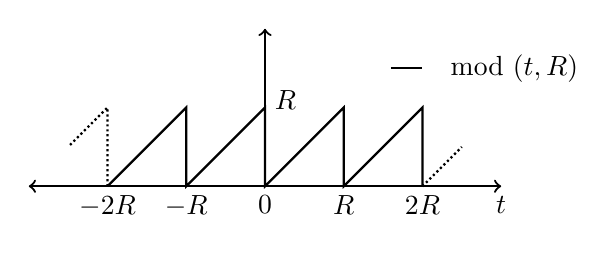
\begin{tikzpicture}
			\draw[<->,thick] (-3,0)--(3,0) node[anchor=north]{$t$};
			\draw (0,0) node[anchor=north]{$0$};
			\draw (0,1.1) node[anchor=west] {$R$};
			\draw (1,0) node[anchor=north]{$R$};
			\draw (2,0) node[anchor=north] {$2R$};
			\draw (-1,0) node[anchor=north]{$-R$};
			\draw (-2,0) node[anchor=north] {$-2R$};
			%\draw [densely dotted,thick] (-2.5,1)--(3,1);
			\draw[->,thick] (0,0)--(0,2);
			\draw[] (2,1.5) node[anchor=west] {{$\mod(t,R)$}};
			\draw[thick] (1.6,1.5) -- (2,1.5);
			\draw[thick] (-2,0) --(-1,1)-| (-1,0) -- (0,1) -| (0,0) --(1,1)-| (1,0) -- (2,1) -| (2,0);
			\draw[densely dotted,thick] (2,0)--(2.5,0.5);
			\draw[densely dotted,thick] (-2,0)|-(-2,1) -- (-2.5,0.5);
			\end{tikzpicture}
	\end{center}
	\caption{\emph{Modulo operation with respect to $R$}}
	\label{fig:orgmodop}
\end{figure}


The standard solution to this issue is to improve sensor dynamic range via enhanced hardware; this, of course, can be expensive. An intriguing alternative is to deploy special digital \emph{modulo} sensors. As the name suggests, such a sensor wraps each signal measurement around a scalar parameter $R$ that reflects the dynamic range. However, this also makes the forward model \eqref{eq:modmeas0} highly nonlinear and the reconstruction problem highly ill-posed. The approach of~\cite{Bhandari,Zhao15} resolves this problem by assuming \emph{overcomplete} observations, meaning that the number of measurements $m$ is higher than the ambient dimension $n$ of the signal itself. For the cases where $m$ and $n$ are large, this requirement puts a heavy burden on computation and storage. 

In contrast, our focus is on solving the the inverse problem~\eqref{eq:modmeas0} with very few number of samples, {i.e.}, we are interested in the case $m \ll n$. While this makes the problem even more ill-posed, we show that such a barrier can be avoided if we assume that the underlying signal obeys a certain low-dimensional structure. In this paper, we focus on the \emph{sparsity} assumption on the underlying signal, but our techniques could be extended to other signal structures.  

%\subsection{Simplified setup}
% CH: this subsection is repetition of the above, probably not necessary
%\label{subsec:setup}
%The $\mod(\cdot,R)$ transfer function is many-to-one with infinite support. Thus, in this paper, we simplify our analysis by considering a simplified version of the modulo function that already inherits much of the challenging aspects of the original function. We consider a modified version that is truncated to only two periods of operation: one on the positive half and one in the negative half as shown in the Fig.~\ref{fig:compare}(a). %We also incorporate sparsity as a signal prior, thus capture the measurements in compressed sense, \textit{i.e.} $m<n$.
%Assume $\mathcal{X} \subseteq \R^n$ to be a given (known) subset in the data space, and consider a signal (or image) $\mb{x}^* \in \mathcal{X}$. We construct $\mathbf{A} = \left[\mathbf{a_1~a_2~...~a_m}\right]^\t$ with i.i.d. Gaussian entries and $m<n$. We aim to recover the original signal $\mb{x^*}\in \R^n$ from its compressed modulo measurements $y_i$, defined as:
%\begin{equation}
%y_i=\mod(\langle \mathbf{a_i} \cdot \mathbf{x^*} \rangle,R)~\textnormal{for}~i = \{1,2,...,m\},
%\label{eq:modmeas1}
%\end{equation} 
%where $\mod(\cdot)$ is modulo operation with respect to a fixed, real-valued parameter $R$. The primary assumption in our model is that the natural signal $\mathbf{x^*}$ is $s-$sparse in a chosen basis. 

%\begin{figure}[h]
%	\begin{center}
%		\begin{tikzpicture}[scale=0.7, every node/.style={scale=0.7}]
%		\draw[<->] (-4,0) -- (4,0) node[right] {$t$};
%		\draw[->] (0,-1) -- (0,4) node[above] {$f(t)$};
%		\draw[scale=0.5, dashed, thick] (0,4)--(7,4) node[right]{$R$};
%		\draw (1.5,-0.5) node(below) {$p_i = 0$};
%		\draw (-1.5,-0.5) node(below) {$p_i = 1$};
%		\draw (0,-1.5) node(right) {$f(t) = \mod(t,R)$};
%		\draw[scale=0.5,domain=-7:0,smooth,variable=\x,blue,thick] plot ({\x},{\x+4});
%		\draw[scale=0.5,domain=0:7,smooth,variable=\x,blue, thick]  plot ({\x},{\x});
%		\end{tikzpicture}
%	\end{center}
%	\caption{\emph{Modified modulo function for the given problem}}
%	\label{fig:modop}
%\end{figure}

\subsection{Our contributions}
In this paper, we propose a recovery algorithm for exact reconstruction of signals from modulo measurements of the form \eqref{eq:modmeas0}. We refer our algorithm as \emph{MoRAM}, short ffor \emph{Modulo Recovery using Alternating Minimization}. The key idea in our approach is to identify and draw parallels between modulo recovery and the problem of \emph{phase retrieval} \todo{include PR citations here}. Indeed, this connection enables us to bring in algorithmic ideas from classical phase retrieval, which also helps in our analysis. 

Phase retrieval has its roots in several classical imaging problems, but has attracted renewed interest of late. There, we are given observations of the form:
\[
y_i= | \langle \mathbf{a_i} , \mathbf{x^*} \rangle|,~~i = 1, 2, \ldots, m,
\]
and are tasked with reconstructing $x^*$.  While these two different class of problems appear different at face value, the common theme is the need of undoing the effect of a piecewise linear transfer function applied to the observations. See Fig.~\ref{fig:compare} for a comparison.
% While we deal with the modified version of modulo function with two periods in the case of modulo recovery, phase retrieval deals with absolute value function which is piece wise linear too. 
%Fig.~\ref{fig:compare} compares both the modulo ($f(t)$) and absolute value ($g(t)$) functions. 
Both the functions are identical to identity function in the positive half, but differs significantly in the negative half. Solving the phase retrieval problem is essentially equivalent to retrieving the phase ($\text{sign}{y_i}$) corresponding to each measurement $y_i$. However, this can take only two values: $1$ if $t \geq 0$, or $-1$ if $t < 0$. Along the same lines, for modulo recovery case, the challenge is to identify the bin-index $p$ for each measurement. %, and can take values $0$ if $t\geq 0$ or $1$ if $t<0$. 
Estimating the bin-index correctly lets us ``unravel'' the modulo transfer function, thereby enabling signal recovery.
\begin{figure}[h]
	\begin{center}
		\begin{tabular}{cc}
			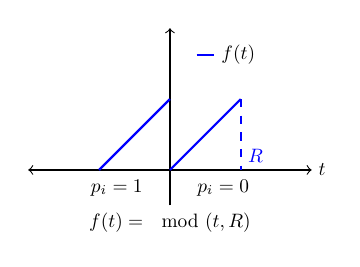
\begin{tikzpicture}[scale=0.45, every node/.style={scale=0.7}]
			\draw[<->] (-4,0) -- (4,0) node[right] {$t$};
			\draw[->] (0,-1) -- (0,4);
			\draw[scale=0.5, dashed, blue, thick] (4,4)--(4,0) node[above right]{$R$};
			\draw (1.5,-0.5) node(below) {$p_i = 0$};
			\draw (-1.5,-0.5) node(below) {$p_i = 1$};
			\draw[scale=0.5,blue,thick] (1.5,6.5)--(2.5,6.5) node[right,black]{$f(t)$};
			%\draw[scale=0.5,dotted,red,ultra thick] (1.5,5.5)--(2.5,5.5) node[right,black]{$g(t)$};
			\draw (0,-1.5) node(right) {$f(t) = \mod(t,R)$};
			\draw[scale=0.5,domain=-4:0,smooth,variable=\x,blue, thick] plot ({\x},{\x+4});
			\draw[scale=0.5,domain=0:4,smooth,variable=\x,blue, thick]  plot ({\x},{\x});
			%\draw[scale=0.5,domain=0:7,smooth,variable=\x,red, ultra thick, dotted]  plot ({\x},{\x});
			%\draw[scale=0.5,domain=-7:0,smooth,variable=\x,red, ultra thick, dotted]  plot ({\x},{-\x});
			\end{tikzpicture} &
			
			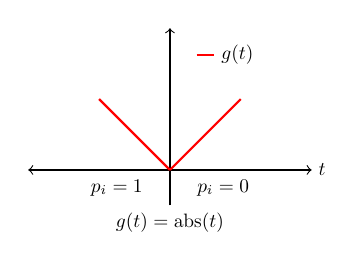
\begin{tikzpicture}[scale=0.45, every node/.style={scale=0.7}]
			\draw[<->] (-4,0) -- (4,0) node[right] {$t$};
			\draw[->] (0,-1) -- (0,4);
			%\draw[scale=0.5, dashed, thick] (0,4)--(7,4) node[right]{$R$};
			\draw (1.5,-0.5) node(below) {$p_i = 0$};
			\draw (-1.5,-0.5) node(below) {$p_i = 1$};
			%\draw[scale=0.5,blue,ultra thick] (1.5,6.5)--(2.5,6.5) node[right,black]{$f(t)$};
			\draw[scale=0.5,red,thick] (1.5,6.5)--(2.5,6.5) node[right,black]{$g(t)$};
			\draw (0,-1.5) node(right) {$g(t)=\mathrm{abs}(t)$};
			%\draw[scale=0.5,domain=-7:0,smooth,variable=\x,blue, ultra thick] plot ({\x},{\x+4});
			%\draw[scale=0.5,domain=0:7,smooth,variable=\x,blue, ultra thick]  plot ({\x},{\x});
			\draw[scale=0.5,domain=0:4,smooth,variable=\x,red,thick]  plot ({\x},{\x});
			\draw[scale=0.5,domain=-4:0,smooth,variable=\x,red, thick]  plot ({\x},{-\x});
			\end{tikzpicture} \\
			(a) & (b)
		\end{tabular}
	\end{center}
	\caption{\emph{Comparison between (a) absolute value function ($g(t) = \mathrm{abs}(t)$) ; and (b) modulo function ($f(t) = \mod(t,R)$)}}
	\label{fig:compare}
\end{figure}

At the same time, several essential differences between the two problems restrict us from using algorithms for phase retrieval as-is for the modulo reconstruction problem. The absolute value function can be represented as a multiplicative transfer function (multiplication with the sign of the measurements), while the modulo function adds a constant value ($R$) to negative inputs. %Value of $p$ denotes whether the $R$ is added in the true measurement or not. It should be noted that the multiplication with $-1$ still preserves the magnitude information of the observations, while the additive process deforms the observation significantly, even more if the value of $R$ is higher. Additionally, the behavior of the modulo function is largely controlled by the value of the parameter $R$, while such parameter is non-existent in the case of absolute value function.
%Therefore, we can measure the effect of such nonlinearity by analyzing the error between true measurements and observed measurements for the negative half of the number-line. 
Therefore, estimation errors propagate very differently in the two cases. In the case of phase retrieval, a wrongly estimated phase induces an error that increases \emph{linearly} with the magnitude of each measurement. %Measurements closer to zero are less affected compared to measurements far from zero. In standard phase retrieval setup, as the true measurements are linear combination of the samples from the Gaussian distribution, resulting distribution of the true measurements follows the Gaussian curve, which makes most of the true measurements concentrate close to zero; lowering the severity of the corruption.
On the other hand, for modulo recovery problem, the error induced by an incorrect bin-index is $R$ (or larger), irrespective of the measurement. Therefore, existing algorithms for phase retrieval perform rather poorly for our problem (both in theory and practice). %Contrary to the case of phase retrieval, here the error is constant irrespective of magnitude of the true measurements. Even the true measurements lying very close to zero would experience the added error of $R$, and thus get severely affected. In the cases where $R$ is large, the magnitude of the additive corruption is way higher than the magnitude of the true measurement. Presence of such noise makes the recovery process very challenging.

We resolve this issue by making non-trivial modifications to existing phase retrieval algorithms that better exploit the structure of modulo reconstruction. We also provide analytical proofs for recoverying the underlying signal using our algorithm, and show that such a recovery can be performed using an (essentially) optimal number of observations, provided certain standard assumptions are met. To the best of our knowledge we are the first to pursue this type of approach for modulo recovery problems, distinguishing us from previous work~\cite{Zhao2015,Bhandari}. 

\subsection{Techniques}

%The proposed MoRAM algorithm is conceptually simple yet novel step in the direction of solving the problem of modulo recovery. Our work takes a fresh approach for solving the modulo recovery problem by borrowing the ideas from the well studied field of phase retrieval and compressive sensing. 
The basic approach in MoRAM is similar to the state-of-the-art phase retrieval approaches. As is the case with most of the non-convex algorithms, in the first step we identify a good initial guess $\mb{x^0}$ for our signal that lies relatively close to the true vector $\mb{x^*}$. A commonly used initialization technique for phase retrieval is \emph{spectral initialization} as described in \cite{Netrapalli2013}. However, that does not work in our case due to variedly different behavior of the modulo transfer function. %However, we observe that the initialization is easier to obtain if we have access to rather a small number of true measurements than having a large number of modulo measurements (corrupted by nonlinearity). 
We introduce a novel approach of measurement \emph{correcting} by comparing with typical histograms of Gaussian observations. Given access to such corrected measurements, $\mb{x^0}$ can be calculated simply by using a first-order estimator. This method is intuitive, yet provides % Our method of recalculating the partial number of true measurements from the set of modulo measurements is intuitive yet gives 
	a provable guarantee for getting a initial vector that is close to the true signal. 

Our second step is to refine this initial estimate to (ideally) provide the true underlying signal. Again, we follow an alternating-minimization (AltMin) approach inspired from the phase retrieval solutions (\cite{Netrapalli2013}) that estimates the signal and the phase alternatively. However, as mentioned above, any estimation errors incurred in the first step induces fairly large additive errors (proportional to the dynamic range parameter $R$.) We resolve this issue by appealing to a \emph{robust} form of alternating minimization (specifically, the Justice Pursuit algorithm~\todo{cite JP}). We prove that AltMin based on Justice Pursuit succeeds provided the number of wrongly estimated bin-indices in the beginning is a small fraction of the total number of measurements. This gives us a natural radius for initialization, and also leads to provable sample-complexity upper bounds.   % In particular,  we use the fact that justice pursuit algorithm manages to correct the corruption in bin-index values, provided the number of corrupted bin-indices is a fraction of total number of measurements. 

\subsection{Paper organization} 
The reminder of the paper is organized as follows. In section~\ref{sec:prior}, we briefly discuss the prior work. Sections~\ref{sec:prelim} contains notation and mathematical model used for our analysis. In section~\ref{sec:algo}, we introduce the MoRAM algorithm, and provide a theoretical analysis of its performance. We demonstrate the performance of our algorithm by providing series of numerical experiments in section~\ref{sec:exp}. Section~\ref{sec:disc} provides concluding remarks.
	\section{Prior work}
\label{sec:prior}
\emph{\textbf{Modulo recovery and phase unwrapping:}} \textcolor{red}{In the literature, typically the modulo recovery problem is considered within the setup of Nyquist sampling \textit{i.e.}, bandlimited (smooth) signal assumption, uniform grid sampling in time/spatial domain etc. being the key characteristics. For example, given the modulo samples of a bandlimited function, \cite{Bhandari} provides a stable algorithm for perfect recovery of the signal and also proves the $O(n)$ sample complexity for the perfect recovery. \cite{Cucuringu2017} formulates and solves an QCQP problem with non-convex constraints for denoising the modulo 1 ($R =1$) samples of the unknown function along with providing a least-square based modulo recovery algorithm. However, both these algorithms consider uniform sampling grid with a bandlimited signal, and thus, not suitable for sparsity based sub-Nyquist sampling scheme. For images, the phase unwrapping algorithm proposed in \cite{bioucas2007phase} (and the subsequent Single-shot UHDR in \cite{ICCP15_Zhao}) is specialized to images, and employs graph cuts for recover true image from a single modulo measurement per pixel. However, the fact that it operates in uniform grid sampling regime with the inherent assumption that the input image has very few sharp discontinuities makes it unsuitable for practical compressive sampling. Our main motivation for this paper is the multi-shot UHDR method of \cite{ICCP15_Zhao}, which reconstructs the true image from multiplexed linear measurements obtained in oversampled setting. There, the measurement matrix has to be chosen carefully, and because the method doesn't use any inherent signal structure, it results in high oversampling factor. In our previous work \cite{Shah}, we proposed an algorithm based on \cite{ICCP15_Zhao, soltani2017stable} for signal recovery from quantized modulo measurements, which can also be adapted for sparse measurements, however, similar to \cite{ICCP15_Zhao}, it doesn't leverage sparsity in the modulo recovery process. Table~\ref{tab:compare} provides a qualitative comparison of our approach with the above mentioned approaches.}

\emph{\textbf{Phase retrieval:}} Approaches to solve phase retrieval problem can be broadly classified into two categories: convex and non-convex. 
Convex approach usually consist of solving a constraint optimization problem after linearizing the problem. PhaseLift algorithm \cite{candes2013phaselift} and its variations \cite{gross2017improved}, \cite{candes2015phasediff} come under this category. Typical non-convex approaches involve finding a good initialization followed by iterative minimization, \textit{e.g.} Approaches based on Amplitude flow \cite{wang2016sparse,wang2016solving} and Wirtinger flow \cite{candes2015phase, zhang2016reshaped,  chen2015solving, cai2016optimal}.

In recent works, phase retrieval problem for the cases where underlying signal is sparse is of growing interest. Some of the convex approaches for sparse phase retrieval includes \cite{ohlsson2012cprl, li2013sparse,bahmani2015efficient,jaganathan2012recovery}. Similarly, non-convex approaches for sparse phase retrieval includes \cite{netrapalli2013phase, cai2016optimal, wang2016sparse}. Our approach in this paper towards solving the modulo recovery problem is mainly inspired from the non-convex sparse phase retrieval framework advocated in \cite{Jagatap2017}. 


%Given the modulo samples of a bandlimited function, \cite{Bhandari} provides a stable algorithm for perfect recovery of the signal and also proves sufficiency conditions that guarantees the perfect recovery. \cite{Cucuringu2017} formulates and solves an QCQP problem with non-convex constraints for denoising the modulo 1 ($R =1$) samples of the unknown function along with providing a least-square based modulo recovery algorithm. However, both these works relay on the smoothness of the bandlimited function as a prior structure on the signal, and can't be used in our setup.

\begin{table*}[t]
	\centering
	\begin{tabular}{|p{4.7cm}|p{3cm}|p{2.2cm}|p{2.6cm}|p{3.2cm}|}
		\cline{1-5}
		& Unlimited Sampling~\cite{Bhandari}& OLS Method~\cite{Cucuringu2018} & multishot UHDR~\cite{ICCP15_Zhao}  & MoRAM \\ \cline{1-5}

		Assumption on structure of signal  & Bandlimited   & Bandlimited &  No assumptions & Sparsity     \\ \cline{1-5}
		Sampling scheme  & uniform grid &  uniform grid  & (carefully chosen) linear measurements   & 
		random linear measurements \\ \cline{1-5}
		Sample complexity & oversampled, $\mathcal{O}(n)$    & --    & oversampled, $\mathcal{O}(n)$   & undersampled,~$\mathcal{O}(slog(n))$ \\ \cline{1-5}
		Provides sample complexity bounds?  & Yes  & --  & No & Yes \\ \cline{1-5}
		Leverages Sparsity?  & No & No   & No    & Yes \\ \cline{1-5}
		(Theoretical) bound on dynamic range    & Unbounded   & Unbounded     & Unbounded   & $2R$  \\ \cline{1-5}                 
	\end{tabular}
\caption{Comparison of different modulo recovery algorithms and corresponding sampling schemes.}
\label{tab:compare}
\end{table*}

%\textcolor{red}{ About comparision between Bhandari et al. and Our approach:: \\
%According to Nyqist-Shannon criterion, a bandlimited signal can be uniquely represented through its samples collected at a sampling frequency twice its bandwidth. Many variations of this theorems are studied, but in most cases the variation arise from the diversity along time dimension, i.e., sparsity vs smoothness or uniform vs non-uniform grid. In Bhandari et al., the theme is varied only based on the amplitude dimension, not on time dimension. It means the setup pertaining to time dimension in Bhandari et al. is same as standard Nyquist sampling set up. This standard setup requires that the signal is smooth in canonical (time/space) basis, and considers uniform grid for sampling. However, the measurement set up along amplitude dimension is modulo. They prove that to recover the signal from the modulo measurements perfectly, the sampling frequency has to be greater than $2e(bandwidth)$.}
%\textcolor{red}{
%Now, just as the Nyquist Shannon sampling and Compressive Sampling is complimentary to each other, ours and Bhandari et al.'s approach seems to be complimentary. Maybe it can be put in this form: In Bhandari et al., the theme is varied only along the amplitude dimension, while in our case, we move away from standard Nyquist sampling by varying the sampling scheme along both the time and amplitude dimension, as we consider both the modulo sampling and sparsity. Also, the method of modulo recovery proposed in Bhandari et al. rely on smoothness, thus cannot be applied in our sparsity based setup. In our case, \textbf{we leverage sparsity for undoing the effect of modulo operation, which is very novel.}}
%
%\textcolor{red}{ About comparision between Tyagi et al. and Our approach:: \\
%The main focus of the work of Tyagi et al. is not the modulo recovery, but the denoising of modulo measurements. However, in the later part of their paper,for completeness, they do provide two different algorithms for modulo recovery once the modulo observations are denoised. Again, the basis of the Tyagi et al. is same as Bhandari at al,  as they also consider a variation along amplitude dimension only (bandlimited signal, smoothness etc. ).Their modulo recovery algorithm rely on smoothness of the function. They do not provide sample complexity bounds as their main focus is on the denoising part. Also, similar to Bhandari et al., the method of modulo recovery proposed in Tyagi et al. rely on smoothness, thus cannot be applied in our sparsity based setup.}
%
%\textcolor{red}{About comparision between Single Shot UHDR, Zhao and Rasker et al.  and Our approach::\\
%	Again, here also the setup is standard Nyquist Shannon, in spatial basis. The key assumption is smoothness of the 'image' in the spatial domain. No sample complexity bounds are provided. similar to Bhandari et al., the method of modulo recovery proposed here also rely on smoothness (in spatial domain, instead of time domain), thus cannot be applied in our sparsity based setup.}
%
%\textcolor{red}{ About comparision between Multi-Shot UHDR, Zhao and Rasker et al.  and Our approach::\\
%	Here, the measurements are taken in spatial domain, but there is no assumption of smoothness. Here the sampling is non-uniform grid (because of the presence of the carefully chosen multipliers implemented through exposure times). In a way it is similar to our setup of non-uniform sampling, but the sparsity  (or any other signal structure) is not leveraged. Thus, the practical sample complexity is very high ( $m$ is at least 2 times the value of $n$). No theoretical analysis provided. This method is compatible to be used with sparsity (as we have used it in our asilomar paper), but the oversampling factor and difficulty in choosing the multipliers are the drawbacks here. Another key difference is: in the modulo recovery process, we are leveraging sparsity directly. Because of sparsity only our recovery is possible. That is better than an approach which doesn't leverage any structure of the signal.}
	\section{Sparse signal recovery}
\label{sec:algo}
Of course, the major challenge is that we do \emph{not} know the bin-index vector. In this section, we describe our algorithm to recover both $\mathbf{x^*}$ and $\mathbf{p^*}$, given $\mathbf{y, A, s, R}$.  Our algorithm \emph{MoRAM (Modulo Reconstruction with Alternating Minimization)} comprises of two stages: (i) an initialization stage, and (ii) descent stage via alternating minimization.

\subsection{Initialization by re-calculating the measurements}
\label{sec:init}

Similar to other non-convex approaches, MoRAM also requires an initial estimate $\mathbf{{x}^0}$ that is close to the true signal $\mathbf{{x}^*}$. We have several initialization techniques available; in phase retrieval, techniques such as spectral initialization are often used. However, the nature of the problem in our case is fundamentally different due to the non-linear \emph{additive} behavior of the modulo transfer function. To overcome this issue, we propose a method to re-calculate the true Gaussian measurements ($\mb{y_c}= \mb{Ax^*}$) from the available modulo measurements. 

The high level idea is to undo the nonlinear effect of modulo operation in a significant fraction of the total available measurements. %To understand the method for such re-calculation, we will first try to understand the effect of modulo operation on the linear measurements.

\subsubsection{Effect of the modulo transfer function} 
\label{sec:modeff}
To provide some intuition, let us first examine the distribution of the $\mathbf{Ax^*}$(Fig.~\ref{fig:hist1}) and $\mathbf{\mod(\mathbf{Ax^*})}$ (shown in Fig.~\ref{fig:hist2}) to understand what information can be obtained from the modulo measurements. We are particularly interested in the case where the elements of $\mathbf{Ax^*}$ are small compared to the modulo range parameter $R$. 

Denote the spread (range) of the linear measurements (entries of $\mathbf{Ax^*}$) with the hyper-parameter $\rho > 0$. We choose a value of $\rho$ such that it bounds the maximum element of $|\mathbf{Ax^*}|$. As shown in Fig.~\ref{fig:hist1}, assuming that the entries of $\mathbf{A}$ are Gaussian, $\mathbf{Ax^*}$ lies within $[-\rho, \rho]$ where $\rho$ can be calculated based on Gaussian tail bounds.

In Fig.~\ref{fig:hist2}, we observe the density plots after passing the linear measurements through modulo operation, assuming that $R>\rho$. Comparing these plots with the distribution of true measurements (Fig.~\ref{fig:hist1}), we can observe how the first density plot transforms into the second when the modulo operation is applied. We can draw the following conclusions:

\begin{itemize}
	\item Only those measurement values lying on the negative side of the x-axis are going to be affected.
	\item Measurement values lying very close to the origin on the negative side of the x-axis in the first density plot would now shift rightwards by $R$, and would occupy values very close to $R$ in the second plot. For $R>\rho$, this region is shaded in green in Fig.~\ref{fig:hist2}. The correct bin-index for the elements in $\mathbf{y}$ with value lying between $\rho$ and $R$ is given by $p^{init}_{i} = 1$.
	\item For $R>\rho$, the density plot of the positive region very close to the origin would remain unaffected. This region is shaded with orange color in Fig.~\ref{fig:hist2}. The correct bin-index for all the elements in $\mathbf{y}$ with value lying between $0$ and $R-\rho$ is given by $p^{init}_{i} = 0$.
	\item Nothing can be immediately concluded for measurements lying in between $(R-\rho)$ to $\rho$. This region is shaded in gray in Fig.~\ref{fig:hist2}. Correct bin-index cannot be identified for this region, so we assign all the elements in $\mathbf{y}$ with value lying between $(R-\rho)$ and $\rho$ as $p^{init}_{i} = 0$. The lower and upper bounds ($t_l$~\&$~t_u$) of this region of uncertainty can be obtained as:
	\begin{align*}
	t_l & = R-\rho, \\
	t_u & = \rho.
	\end{align*}
	%\item Irrespective of relationship between $\rho$ and $R$, all the values lying in the negative half of the real line have the bin-index equal to $1$, and all the values greater than $R$ have the bin-index equal to $0$.
\end{itemize}

\begin{algorithm}[!t]
	\caption{\textsc{MoRAM-initialization}}
	\label{alg:RCM}
	\begin{algorithmic}
		\State\textbf{Inputs:} $\mathbf{y}$, $\mathbf{A}$, $s$, $R$, $\rho$
		\State\textbf{Output:}  $\mb{x^0}$
		\State $U \leftarrow \emptyset$%, $t_l \leftarrow (R-\rho)$, $t_u \leftarrow R$
		\For {$i= 0:m$}
		%		\If {$y_l<0$}
		%		\State {$p^{rcm}_l = 1$, $T \leftarrow T \cup {l}$}
		%		\ElsIf {$0\leq y_l < t_l$}
		%		\State {$p^{rcm}_l = 0$, $T \leftarrow T \cup {l}$}
		%		\ElsIf {$t_l\leq y_l < t_u$}
		%		\State {$p^{rcm}_l = 0$}
		%		\ElsIf {$t_u \leq y_l < R$}
		%		\State {$p^{rcm}_l = 1$, $T \leftarrow T \cup {l}$}
		%		\ElsIf {$R  \leq y_l$}
		%		\State {$p^{rcm}_l = 0$, $T \leftarrow T \cup {l}$}
		%		
		%		\EndIf
		
		\If {$(R-\rho) > y_i$ or $ y_i \geq \rho$}
		\State {$U \leftarrow U \cup \{i\}$}
		\EndIf
		\State Calculate $p^{init}_i$ according to Eq.~\ref{eq:rcm}.
		\EndFor
		\State $N \leftarrow |U|$, calculate $\mb{y^{init}_c}$ according to Eq.~\ref{eq:init}:
		\State $$\mb{x^0} \leftarrow H_s\left( \frac{1}{N}\sum_{i=1}^{N}y^{init}_{c,U,i}a_{U,i}\right)$$
	\end{algorithmic}
\end{algorithm}


\begin{figure}[!t]
	\begin{center}
		\begin{tikzpicture}[scale=0.7, every node/.style={scale=0.7}]
		\def\normaltwo{\x,{3*1/exp(((\x)^2)/2)}}
		\def\y{4.4}
		
		%\fill [fill=orange!60] (2.6,0) -- plot[domain=0:4.4] (\normaltwo) -- ({\y},0) -- cycle;
		
		% Draw and label normal distribution function
		\draw[color=blue,domain=-4.25:4.25,thick] plot (\normaltwo) node[right] {};
		\draw[<->] (-5,0) -- (5,0) node[right] {$\mathbf{Ax^*}$};
		\draw[<->] (0,-1) -- (0,4);
		
		\draw (-3,-0.5) node(below) {$-\rho$};
		\draw (-4,-0.5) node(below) {$-R$};
		\draw (3,-0.5) node(below) {$\rho$};
		\draw (4,-0.5) node(below) {$R$};
		
		\foreach \x in {-3,-4,3,4}
		{        
			\coordinate (A\x) at ($(0,0)+(\x*1cm,0)$) {};
			\draw ($(A\x)+(0,5pt)$) -- ($(A\x)-(0,5pt)$);
			
		}
		%		\draw (-1.5,-0.5) node(below) {$p_i = 1$};
		%		\draw (0,-1.5) node(right) {$f(t) = \mod(t,R)$};
		%		\draw[scale=0.5,domain=-7:0,smooth,variable=\x,blue, ultra thick] plot ({\x},{\x+4});
		%		\draw[scale=0.5,domain=0:7,smooth,variable=\x,blue, ultra thick]  plot ({\x},{\x});
		\end{tikzpicture}
	\end{center}
	\caption{\emph{Density plot of $\mathbf{Ax^*}$}}
	\label{fig:hist1}
\end{figure}

\begin{figure}[!t]
	\begin{center}
		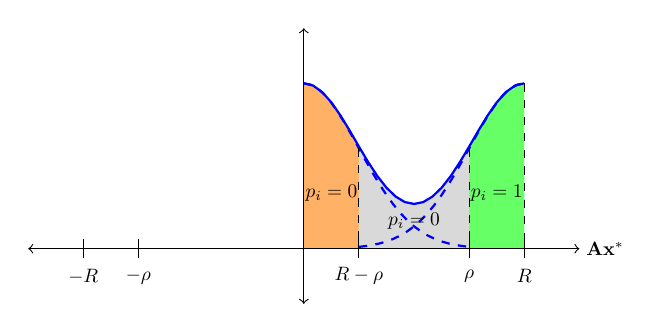
\begin{tikzpicture}[scale=0.7, every node/.style={scale=0.7}]
		\def\normaltwo{\x,{3*1/exp(((\x)^2)/2)}}
		\def\normalone{\x,{3*1/exp(((\x-4)^2)/2)}}
		\def\normalsum{\x,{3*1/exp(((\x-4)^2)/2)+3*1/exp(((\x)^2)/2)}}
		\def\y{3}
		\def\fy{3*1/exp(((\y-4)^2)/2)}
		\fill [fill=orange!60] (0,0) -- plot[domain=0:1] (\normaltwo) -- (1,0) -- cycle;
		\fill [fill=green!60] (3,0) -- plot[domain=3:4] (\normalone) -- (4,0) -- cycle;
		\fill [fill=gray!30] (1,0) -- plot[domain=1:3] (\normalsum) -- (3,0) -- cycle;
		% Draw and label normal distribution function
		\draw[color=blue,domain=-0:3,dashed,thick] plot (\normaltwo) node[right] {};
		\draw[color=blue,domain=1:4,dashed,thick] plot (\normalone) node[right] {};
		\draw[color=blue,domain=-0:4,thick] plot (\normalsum) node[right] {};
		\draw[<->] (-5,0) -- (5,0) node[right] {$\mathbf{Ax^*}$};
		\draw[<->] (0,-1) -- (0,4);
		\draw[dashed] ({\y},{\fy}) -- ({\y},0);
		\draw[dashed] ({4},{3}) -- ({4},0);
		\draw[dashed] ({1},{\fy}) -- ({1},0);
		\draw (-3,-0.5) node(below) {$-\rho$};
		\draw (-4,-0.5) node(below) {$-R$};
		\draw (3,-0.5) node(below) {$\rho$};
		\draw (4,-0.5) node(below) {$R$};
		\draw (1,-0.5) node(below) {$R-\rho$};
		\draw (0.5,1) node(below) {$p_i=0$};
		\draw (3.5,1) node(below) {$p_i=1$};
		\draw (2,0.5) node(below) {$p_i=0$};
		\foreach \x in {-3,-4,1,3,4}
		{        
			\coordinate (A\x) at ($(0,0)+(\x*1cm,0)$) {};
			\draw ($(A\x)+(0,5pt)$) -- ($(A\x)-(0,5pt)$);
			
		}
		%		\draw (-1.5,-0.5) node(below) {$p_i = 1$};
		%		\draw (0,-1.5) node(right) {$f(t) = \mod(t,R)$};
		%		\draw[scale=0.5,domain=-7:0,smooth,variable=\x,blue, ultra thick] plot ({\x},{\x+4});
		%		\draw[scale=0.5,domain=0:7,smooth,variable=\x,blue, ultra thick]  plot ({\x},{\x});
		\end{tikzpicture}
	\end{center}
	\caption{\emph{Density plot of $\mod(\mathbf{Ax^*})$, $R>\rho$}. Best viewed in color.}
	\label{fig:hist2}
\end{figure}
%
%\begin{figure}[!h]
%	\begin{center}
%		\begin{tikzpicture}[scale=0.7, every node/.style={scale=0.7}]
%		\def\normaltwo{\x,{3*1/exp(((\x)^2)/2)}}
%		\def\normalone{\x,{3*1/exp(((\x-2)^2)/2)}}
%		\def\normalsum{\x,{3*1/exp(((\x-2)^2)/2)+3*1/exp(((\x)^2)/2)}}
%		\def\y{3}
%		\def\fy{3*1/exp(((\y-4)^2)/2)}
%		\fill [fill=orange!60] (-1,0) -- plot[domain=-1:0] (\normalone) -- (0,0) -- cycle;
%		\fill [fill=green!60] (2,0) -- plot[domain=2:3] (\normaltwo) -- (3,0) -- cycle;
%		\fill [fill=gray!30] (0,0) -- plot[domain=0:2] (\normalsum) -- (2,0) -- cycle;
%		% Draw and label normal distribution function
%		\draw[color=blue,domain=-0:3,dashed,thick] plot (\normaltwo) node[right] {};
%		\draw[color=blue,domain=-1:2,dashed,thick] plot (\normalone) node[right] {};
%		\draw[color=blue,domain=-0:2,thick] plot (\normalsum) node[right] {};
%		\draw[<->] (-5,0) -- (5,0) node[right] {$\mathbf{Ax^*}$};
%		\draw[<->] (0,-1) -- (0,4);
%		%\draw[dashed] ({\y},{\fy}) -- ({\y},0);
%		\draw[dashed] ({-1},{2}) -- ({-1},0);
%		\draw[dashed] ({3},{2}) -- ({3},0);
%		%\draw[dashed] ({1},{\fy}) -- ({1},0);
%		\draw (-3,-0.5) node(below) {$-\rho$};
%		\draw (-2,-0.5) node(below) {$-R$};
%		\draw (3,-0.5) node(below) {$\rho$};
%		\draw (2,-0.5) node(below) {$R$};
%		\draw (-1,-0.5) node(below) {$-\rho+R$};
%		\draw (-0.5,1) node(below) {$p_i=0$};
%		\draw (2.5,1) node(below) {$p_i=1$};
%		\draw (1,0.5) node(below) {$p_i=0$};
%		\foreach \x in {-3,-2,-1,3,2}
%		{        
%			\coordinate (A\x) at ($(0,0)+(\x*1cm,0)$) {};
%			\draw ($(A\x)+(0,5pt)$) -- ($(A\x)-(0,5pt)$);
%			
%		}
%		%		\draw (-1.5,-0.5) node(below) {$p_i = 1$};
%		%		\draw (0,-1.5) node(right) {$f(t) = \mod(t,R)$};
%		%		\draw[scale=0.5,domain=-7:0,smooth,variable=\x,blue, ultra thick] plot ({\x},{\x+4});
%		%		\draw[scale=0.5,domain=0:7,smooth,variable=\x,blue, ultra thick]  plot ({\x},{\x});
%		\end{tikzpicture}
%	\end{center}
%	\caption{\emph{Histogram of $\mod(\mathbf{Ax^*})$, $R<\rho$}}
%	\label{fig:hist3}
%\end{figure}
We divide the number line in the following $3$ intervals, and assign the bin-index accordingly:
\begin{equation}
{p}^{init}_{i} = 
\begin{cases}
%1,& \text{if } y_i <0 \\
0,& \text{if } 0\leq y_i < t_l \\
0,& \text{if } t_l\leq y_i < t_u ~~~~ \textnormal{(region of uncertainty)} \\
1,& \text{if } t_u \leq y_i < R \\
%0,& \text{if } R  \leq y_i. \\
\end{cases}
\label{eq:rcm}
\end{equation}
Therefore, we can identify the correct bin-index for a significant fraction of the measurements by merely observing their magnitude. We define set $U$ as the set of measurements for which we can identify the bin-index correctly. If $N=: \card(U)$, then we have:
\begin{align*}
N & =  m - \card(\textnormal{measurements within region of uncertainty}).
\end{align*}
The value of $N$ largely depends on the difference between $\rho$ and $R$.

Once we identify the correct bin-index for a portion of the measurements, we can undo the modulo operation by introducing a measurement \emph{correction} step as:
$$
\mathbf{y^{init}_{c} = y + p^{init}R}.
$$
We use these corrected measurements $\mathbf{y^{init}_c}$ to calculate the initial estimate $\mathbf{{x}^0}$ as follows.

\subsubsection{Calculating the initial estimate from the corrected measurements}
In the estimation step, $\mb{x^0}$ is calculated only from the $N$ corrected measurements using a simple first-order unbiased estimator. For that, we use the versions of $\mb{y}$ and $A$ truncated to the indices belong to set $U$:
\begin{equation}
\mb{x^0} = H_s\left( \frac{1}{N}\sum_{i=1}^{N}y^{init}_{c,U,i}a_{U,i}\right),
\label{eq:init}
\end{equation}
where $H_s$ denotes the hard thresholding operator that keeps the $s$ largest absolute entries of a vector and sets the other entries to zero.


\subsection{Alternating Minimization}
\label{sec:altmin}
\begin{algorithm}[t]
	\caption{\textsc{MoRAM-descent}}
	\label{alg:MoRAM}
	\begin{algorithmic}
		\State\textbf{Inputs:} $\mathbf{y}$, $\mathbf{A}$, $s$, $R$
		\State\textbf{Output:}  $\mb{x^T}$
		\State $m,n \leftarrow \mathrm{size}(\mathbf{A})$ 
		\State \textbf{Initialization}
		\State $\mathbf{x^0} \leftarrow \textrm{MoRAM-initialization}(\mathbf{y, A})$ 
		\State \textbf{Alternating Minimization}
		\For {$t =0:T$}
		\State $\mathbf{{p}^{t}} \leftarrow \frac{\mathbf{1}-\sgn(\langle \mathbf{A} \cdot \mathbf{x^t} \rangle)}{2}$
		\State $\mathbf{y^t_c} \leftarrow \mathbf{y} - \mathbf{p^t}R$
		\State $\mathbf{{x}^{t+1}}\leftarrow \small{JP(\frac{1}{\sqrt{m}}\begin{bmatrix} \mathbf{A} & \mathbf{I} \end{bmatrix},\frac{1}{\sqrt{m}}\mathbf{y^t_c},[\mathbf{x^t~~p^t}]^\t)}$.
		\EndFor
	\end{algorithmic}
\end{algorithm}

Using Eq.~\ref{eq:init}, we calculate the initial estimate of the signal $\mathbf{{x}^0}$ which is relatively close to the true vector $\mathbf{x^*}$. Starting with $\mathbf{{x}^0}$, we calculate the estimates of $\mathbf{p}$ and $\mathbf{x}$ in an alternating fashion to converge to the original signal $\mathbf{x^*}$. At each iteration of alternating-minimization, we use the current estimate of the signal ${\mathbf{x^t}}$ to get the value of the bin-index vector $\mathbf{{p}^t}$ as following:
\begin{equation}
\mathbf{{p}^{t}} = \frac{\mathbf{1}-\sgn(\langle \mathbf{A} \cdot \mathbf{x^t} \rangle)}{2}.
\label{step1}
\end{equation}

Given that $\mathbf{x^0}$ is close to $\mathbf{x^*}$, we expect that $\mathbf{p^0}$ would also be close to $\mathbf{p^*}$. Ideally, we would calculate the correct compressed measurements $\mathbf{y^t_c}$ using $\mathbf{p^t}$, and use $\mathbf{y^t_c}$ with any popular compressive recovery algorithms such as CoSaMP or basis pursuit to calculate the next estimate $\mathbf{{x}^{t+1}}$. Thus,

$$
\mathbf{y^t_c} = \langle \mathbf{A}\mathbf{x^{t+1}} \rangle = \mathbf{y} - \mathbf{p^t}R,
$$

$$
\mathbf{{x}^{t+1}} = \argmin_{\mathbf{x} \in \mathcal{M}_s}\norm{\mathbf{Ax} - \mathbf{y^t_c}}_2^2, %~~\mathrm{s.to}~~x^* \in \mathcal{M}_s,
$$
%\begin{equation}
%\implies \mathbf{{x}^{t+1}} = \cosamp(\frac{1}{\sqrt{m}}\mathbf{A},\frac{1}{\sqrt{m}}\mathbf{y^t_c},s,\mathbf{x^t}).
%\label{eq:cosamp}
%\end{equation}
where $\mathcal{M}_s$ denotes the set of $s$-sparse vectors in $\mathbb{R}^n$. Note that sparsity is only one of several signal models that can be used here, and in principle a rather similar formulation would extend to cases where $\mathcal{M}$ denotes any other structured sparsity model~\cite{modelcs}.

However, it should be noted that the ``bin'' error $\mathbf{d^t} = \mathbf{p^t - p^*}$, even if small, would significantly impact the correction step that constructs $\mathbf{y^t_c}$, as each incorrect bin-index would add a noise of the magnitude $R$ in $\mathbf{y^t_c}$. Our experiments suggest that the typical sparse recovery algorithms are not robust enough to cope up with such large errors in $\mathbf{y^t_c}$. To tackle this issue, we employ an outlier-robust sparse recovery method \cite{Laska2009}. We consider the fact that the nature of the error $\mathbf{d^t}$ is sparse with sparsity $s_{dt}=\norm{\mb{d^t}}_0$; and each erroneous element of $\mathbf{p}$ adds a noise of the magnitude $R$ in $\mathbf{y^t_c}$.

Rewriting in terms of Justice Pursuit, the recovery problem now becomes problem becomes,

$$
\mathbf{{x}^{t+1}}=\argmin_{[\mathbf{x~d}]^\t \in \mathcal{M}_{s+s_{dt}}}\norm{\begin{bmatrix} \mathbf{A} & \mathbf{I} \end{bmatrix} \begin{bmatrix} \mathbf{x} \\ \mathbf{d} \end{bmatrix} - \mathbf{y^t_c}}_2^2, %~~\mathrm{s.to}~~x^* \in \mathcal{M}_s,
$$
%\begin{equation}
%= \cosamp(\frac{1}{\sqrt{m}}\begin{bmatrix} \mathbf{A} & \mathbf{I} \end{bmatrix},\frac{1}{\sqrt{m}}\mathbf{y_c^t},s+s_p,[\mathbf{x^t~~p^t}]^\t).
%\label{eq:robcosamp}
%\end{equation}

 However, the sparsity of $\mathbf{d^t}$ is unknown, suggesting that greedy sparse recovery methods cannot be directly used without an additional hyper-parameter. Thus, we employ basis pursuit~\cite{candes2006compressive} which does not rely on sparsity. The robust formulation of basis pursuit is referred as Justice Pursuit (JP) \cite{Laska2009}, specified in Eq.~\ref{eq:jp}.
\begin{equation}
\implies \mathbf{{x^{t+1}}} = JP(\frac{1}{\sqrt{m}}\begin{bmatrix} \mathbf{A} & \mathbf{I} \end{bmatrix},\frac{1}{\sqrt{m}}\mathbf{y^t_c},[\mathbf{x^t~~p^t}]^\t).
\label{eq:jp}
\end{equation}
Proceeding this way, we repeat the steps of bin-index calculation (as in Eq.~\ref{step1}) and sparse recovery (Eq.~\ref{eq:jp}) altenatingly for $\mathrm{T}$ iterations. Our algorithm is able to achieve convergence to the true underlying signal, as supported by the results in the experiments section.

%Thus, we can have two variants of the MoRAM algorithm: (i) MoRAM with CoSaMP, (ii) MoRAM with robust CoSaMP, and (iii) MoRAM with Justice Pursuit. 

%$$
%\norm{\begin{bmatrix} \mathbf{A} & \mathbf{I} \end{bmatrix} \begin{bmatrix} \mathbf{x^*} \\ \mathbf{d} \end{bmatrix} - \mathbf{y}}_2^2.
%$$

%

	\newpage

\section{Mathematical Analysis}

\subsection{Analysis of the Initialization}
We perform the initialization in two steps:
(i) Measurement correction step, (ii) Estimation step.

\subsubsection{Measurement correction step}: In this step, based on the absolute value of the modulo measurements, we identify the measurements for which we can undo the effect of the modulo operation by guessing the correct value of $\mathbf{p}$. We define the set $T$ as set of indices of all such measurements.

We determine the measurements to be corrected based on the method described in section~{\todo{add section}}. 
In this analysis, our goal is to find out the total number of measurements ($N=|T|$), that can be corrected through the \todo{histogram analysis -  change the term}. Only these $N$ measurements would be used in the estimation step.
Each element of $A$ id i.i.d. standard normal, thus, $\mu_{A_{ij}} = 0$ and $\sigma_{A_{ij}}=1$.
$$
y_{c,i} =\langle \mathbf{a_i} \cdot \mathbf{x^*} \rangle = \sum_{j=1}^{n}A_{ij}x^*_{j}.
$$

So, 
$$
y_{c,i} \sim \mathcal{N}\left(\mu= \sum_{j=1}^{n}x^{*}\mu_{A_{ij}}, \sigma =\sum_{j=1}^{n}x^{*2}_{j}\sigma^2_{A_{ij}}\right)
$$
$$
\implies y_{c,i} \sim \mathcal{N}\left(\mu= 0, \sigma =\sum_{j=1}^{n}x^{*2}_{j} = \norm{\mathbf{{x}^*}}^2 = 1 \right)
$$

Here, each element of $\mathbf{y_c}$ follows a zero mean Gaussian distribution with unit variance.

Now to calculate $N$, we consider the following result:
We can calculate $N$ using the fact that the measurements follow the standard normal distribution, and the total number of measurements are $m$.
Number of measurements lying in the interval $[\alpha,\beta]$ = $mP(\alpha \leq y_{c,i}\geq \beta) = m\left(Q(\alpha)- Q(\beta)\right)$; \\
Where, $Q(\cdot)$ is Q-function, defined as, $Q(t) = 1-\Phi(t)$ with $\Phi(\cdot)$ being CDF of standard normal distribution. \\
We also note that $Q(-t) = 1 - Q(t)$. \\
Q-function is not an elementary function. However, it can be bounded by following functions where $\phi(\cdot)$ is standard normal density function:
$$
\left(\frac{t}{1+t^2}\right)\phi(t) < Q(t) < \frac{\phi(t)}{t}.
$$

case (i) $R > \rho$: in this case, \\
$N$ = number of measurements lying in the interval $[-R + \rho,0]$ + number of measurements lying in the interval $[0, R-\rho]$.
\begin{equation}
N = m\left(Q(-R+\rho)- Q(0)\right) + m\left(Q(0)- Q(R-\rho)\right)
~~ = m\left(Q(-(R-\rho))- Q(R-\rho)\right) 
~~ = m\left(1-2Q(R-\rho)\right)
\end{equation}

Using the above bounds,
$$
N \geq m \left(1-2\frac{\phi(R-\rho)}{(R-\rho)} \right)
$$

case (ii) $R < \rho$: in this case, \\
$N$ = number of measurements lying in the interval $[-\rho,-R]$ + number of measurements lying in the interval $[R,\rho]$.
\begin{equation}
N = m\left(Q(-\rho)- Q(-R)\right) + m\left(Q(R)- Q(\rho)\right)
~~ = m\left(1 - Q(\rho)-1 +Q(R) +Q(R) -Q(\rho)\right) 
~~ = 2m\left(Q(R)-Q(\rho)\right)
\end{equation}

Using the above bounds,
$$
N \geq 2m \left(\frac{R}{(1+R^2)} \phi(R) - \frac{\phi(\rho)}{\rho}\right)
$$


\subsubsection{Estimation step}

We calculate the initial estimate using the measurements in set $T$ as following,
$$
\mathbf{{x}^0} = M = \frac{1}{|T|}\sum_{i\in T}y_{i}a_{i}.
$$

We use the versions of $\mb{y}$ and $A$ truncated to the indices belong to set $T$.
$$
\mathbf{{x}^0} = M = \frac{1}{N}\sum_{i=1}^{N}y_{T,i}a_{T,i} =  \frac{1}{N}A^T\mb{y_T}.
$$
Substituing $\mb{y_T}=A_T\mb{x^*}$,
$$
\mathbf{{x}^0} = M = \frac{1}{N}A_T^\t A_T\mb{x^*}.
$$

We note that each row of our Gaussian measurement matrix ($A_{T,i}$) is independent, and also follows the Guassian distribution with zero mean.  
We denote this distribution with Gaussian random vector $Z$ in $\R^n$, and arrange $N$ rows as the independent samples from the distribution; $Z_i := A_{T,i}$. 

Recall that the covariance matrix of $Z$ can be calculated as $\Sigma = \mathbb{E}Z\otimes Z$,
$$
\Sigma= \mathbb{E}Z\otimes Z = \mathbb{E} ZZ^\t = diag(\mathbb{E}z_1^2,\mathbb{E}z_2^2,...,\mathbb{E}z_n^2) = I_n
$$

Now, calculating the sample covariance matrix of $Z$ using the samples $Z_i = A_{T,i}$,
$$
\Sigma_N = \frac{1}{N}\sum_{i=1}^{N}Z_i \otimes Z_i = \frac{1}{N} A_T^\t A_T
$$
Let $\epsilon \in (0,1), t\geq 1$,
We invoke the Corrolary 5.50 of \cite{} \todo{cite vershynin},
\theorem{Let $\epsilon\in (0,1)$ and $t \geq 1$. The initial estimate $\mb{x^0}$ is the output of the algorithm \todo{add algo ref}. If the total number of corrected measurements satisfy, $N \geq C(\frac{t}{\epsilon})^2n$, then  with probability at least $1 - 2\exp\left(-t^2n\right)$ we have,
$$
\norm{\mb{x^0} - \mb{x^*}}_2 \leq \epsilon \norm{\mb{x^*}}_2.
$$
}

\begin{align*}
\norm{\Sigma_N - \Sigma} &\leq \epsilon \\
\implies \norm{\frac{1}{N} A_T^\t A_T - I_n} &\leq \epsilon \\
\implies \sup_{\mb{x} \in \R^n} \frac{\norm{\left(\frac{1}{N} A_T^\t A_T - I_n\right)\mb{x}}_2}{\norm{\mb{x}}_2} &\leq \epsilon \\
\implies \norm{\left(\frac{1}{N} A_T^\t A_T - I_n\right)\mb{x^*}}_2 &\leq \epsilon \norm{\mb{x^*}_2} \\
\implies \norm{\left(\frac{1}{N} A_T^\t A_T\mb{x^*} - \mb{x^*}\right)}_2 &\leq \epsilon \norm{\mb{x^*}_2} \\
\implies \norm{\mb{x^0} - \mb{x^*}}_2 &\leq \epsilon \norm{\mb{x^*}}_2 \\
\end{align*}


\subsection{Analysis of the Convergence}
We perform the Alternative Minimization Algorithm as described in~\ref{alg:MoRAM}, starting with $\mb{x^0}$ calculated as above. 
The first step is to obtain the initial estimate for bin-index vector, $\mb{p^0}$ using $\mb{x^0}$.
$$
\mathbf{{p}^{0}} = \frac{\mathbf{1}-\sgn(\langle \mathbf{A} \cdot \mathbf{x^0} \rangle)}{2}.
$$
If we try to undo the effect of modulo operation by adding back $R$ for the affected measurements based on the bin-index vector $\mb{p^0}$, it would introduce the error equaling $R$ corresponding to the incorrect bin-index values in $\mb{p^0}$.
$$
\mathbf{y^0_c} = \langle \mathbf{A}\mathbf{x^{0}} \rangle = \mathbf{y} - \mathbf{p^0}R,
$$

If the initial bin-index vector $\mb{p^0}$ is close to the true bin-index vector $\mb{p^*}$, then the fraction of noisy measurements in $\mb{y^0_c}$ with respect to total number of measurements $m$ is small enough to treat $\mb{y^0_c}$ as sparsely corrupted measurements. Unlike the general cases of noise, in this case the corruption cannot be modeled as a probability distribution. However, if we model this corruption as a sparse noise, then we can employ Justice Pursuit for a guaranteed recovery of the true signal given (i) sparsity of the noise is a fraction of total number of measurements; (ii) sufficiently large number of measurements are available. In the following theorem, we claim the guaranteed recovery of the true signal as the corruption in the first set of corrected measurements $\mb{y_c^0}$ can be modeled as sparse vector with sparsity less than or equal to $Cm$, with $C$ being a fraction. 

\lemma{Let $\mb{A}$ be the matrix generated as $\mb{A} \sim \mathcal{N}^{m \times n}(0,1)$ and $\mb{x^*, x^0} \in \R^n$ are $s-$sparse vectors satisfying $\norm{\mb{x^* - x^0}}_2 \leq \delta_1$. Let $\epsilon \in (0,1)$. Given the number of measurements $m \geq ***$, following is true with probability exceeding $1 - (****)$:
	
	$$
	d_H(\sgn({\mb{Ax^*}}), \sgn({\mb{Ax^0}})) \leq \delta_1 + \epsilon;
	$$
where $d_H$ is Hamming distance between binary vectors defined as:

$$
d_H(\mb{a,b}) =: \frac{1}{n}\sum_{i=1}^{n}a_i \oplus b_i \textnormal{~~for $n-$ dimensional binary vectors~} \mb{a,b}.
$$ 
}
\textit{Proof.} For proof, we first introduce the concept of binary $\epsilon$-stable embedding as appears in \todo{cite jacques}.
\definition[Binary $\epsilon$-Stable Embedding]{A mapping $F: \R^n \rightarrow \mathcal{B}^m$ is a binary $\epsilon$-stable embedding (B$\epsilon$SE) of order $s$ for sparse vectors if:
$$
d_S(\mb{x,y}) - \epsilon \leq d_H(F\mb{(x)},F\mb{(y)}) \leq d_S(\mb{x,y}) + \epsilon;
$$
for all $\mb{x,y} \in S^{n-1}$ with $|supp(x) \cup supp(y)|\leq s$.
}
 
In our case, let's define the mapping $F: \R^n \rightarrow \mathcal{B}^m$ \todo{add definition of Bm} as:
$$
F(\mb{x})=: \sgn(\mb{Ax});
$$
with $\mb{A} \sim \mathcal{N}^{m \times n}(0,1)$.

Given $m > ****$, using Theorem 3 from \todo{cite jacques} we conclude that $F$ is a B$\epsilon$SE for $s$-sparse vectors.
Thus for sparse vectors $\mb{x^*, x^0}$:
$$
d_H(F\mb{(x^*)},F\mb{(x^0)}) \leq d_S(\mb{x^*,x^0}) + \epsilon
$$

$$
\implies d_H(\sgn({\mb{Ax^*}}), \sgn({\mb{Ax^0}})) \leq \delta_1 + \epsilon.
\qed
$$


\todo{conversion from angle to l2 distance}

\theorem{Given an initialization $\mb{x^0}$ satisfying $\norm{\mb{x^* - x^0}}_2 \leq \delta_1\norm{\mb{x^*}}_2$, for $0 < \delta_1 < 1$, if we have number of (Gaussian) measurements $m > ****$ , then the iterates of Algorithm \ref{alg:MoRAM} satisfy:
$$
\norm{\mb{x^{t+1} - x^*}}_2 \leq \rho_0 \norm{\mb{x^t}-\mb{x^*}}_2,
$$
with probability greater than $1-****$, for $0<\rho_0<1$.
}

\textit{Proof.} We compute the corruption in $\mb{y_c^0}$ as,

$$
\eta = \mb{y_c^0 - y_c} = \mathbf{y} - \mathbf{p^0}R - \mathbf{y} + \mathbf{p^*}R = (\mb{p^*-p^0})R = \Delta\mb{p}R.
$$

Expanding further,
\begin{align*}
\eta  & = \frac{\mathbf{1}-\sgn(\langle \mathbf{A} \cdot \mathbf{x^0} \rangle)}{2} -  \frac{\mathbf{1}-\sgn(\langle \mathbf{A} \cdot \mathbf{x^*} \rangle)}{2} \\
& = \frac{\sgn({\mb{Ax^*}})- \sgn({\mb{Ax^0}})}{2} \\
& = \frac{F\mb{(x^*)} - F\mb{(x^0)}}{2} \\
& = d_H(F\mb{(x^*)}, F\mb{(x^0)}) \\
& \leq \delta_1 + \epsilon = C_1m.
\end{align*}

Justice Pursuit formulation is used to recover the signal in th
	\section{Numerical experiments}
\label{sec:exp}
In this section, we present the results of simulations of signal reconstruction using our algorithm. All numerical experiments were conducted using MATLAB R2017a on a linux system with an Intel CPU and 64GB RAM. Our experiments explores the performance of the MoRAM algorithm on both synthetic data as well as real images.

We perform experiments on a synthetic sparse signal $\mb{x^*} \in \R^n$ generated randomly with $n=1000$. The sparsity level of the signal is chosen in steps of $3$ starting from $3$ with a maximum value of $12$. The non-zero elements of the test signal $\mb{x^*}$ are generated using zero-mean Gaussian distribution $\mathcal{N}(0, 1)$ and normalized such that $\norm{\mb{x^*}} =1$. The elements of the Gaussian measurement matrix $\mb{A} \in \R^{m\times n}, a_{ij}$ are also generated using the standard normal distribution $\mathcal{N}(0, 1)$. The number of measurements $m$ is varied from $m = 100$ to $m=1000$ in steps of $100$.  

It is important to note that unlike the absolute value function, the modulo function described in Fig.~\ref{fig:graph} is not scale-invariant. The modulo function works over the quantities $y_{c,i}=\langle \mathbf{a_i} \cdot \mathbf{x^*} \rangle, i=1,..,m$; and it is defined over the parameter $R$; thus depending on the magnitudes of $y_{c,i}$ and $R$ relative to each other, the behavior of the measurement model and the reconstruction algorithm would be altered. For instance, if the value of $R$ is too small compared to the range of the $y_{c,i}$, the modulo operation would hardly have any effect on the measurements, leaving $\mathbf{y_c \approx y}$. To analyze such variations, we fix the signal strength by setting $\norm{\mb{x^*}} =1$ in our experiments, while varying the value of modulo parameter $R$ as ${1,2,4}$.

Using $\mb{A, x^*}$ and $\R$, We first obtain the compressed modulo measurements $\mb{y}$ by passing the signal through forward model described by Eq.~\ref{eq:modmeas2}. We compute the initial estimate $\mathbf{x^0}$ using the algorithm~\ref{alg:RCM}. For reconstruction, algorithm~\ref{alg:MoRAM} is employed. we plot the variation of the relative reconstruction error ($\frac{\norm{\mathbf{x^*-x^N}}}{\norm{\mathbf{x^*}}}$) with number of measurements $m$ for our AltMin based sparse recovery algorithm MoRAM.

For each combination of $R, m$ and $s$, we run $10$ independent Monte Carlo trials, and calculate mean of the relative reconstruction error over these trials. Figs.~\ref{fig:plot-r-1},~\ref{fig:plot-r-2} and~\ref{fig:plot-r-4} illustrate the performance of our algorithm for increasing values of $R$ respectively. It is evident that for each combination of $R$ and $s$, our algorithm converges with probability $1$ to give the exact recovery of the true signal (zero relative error) provided enough number of measurements. In all such cases, the minimum number of measurements required for exact recovery are well below the ambient dimension $(n)$ of the underlying signal. 

%Another important factor affecting the reconstruction is the quality of the initial estimate ($\mathbf{{x}^0}$) obtained through first order estimation. As described in~\ref{sec:init}, the quality of the initial estimate is a direct function of number of measurements ($m$). As we set $m$ higher, the initial estimate $\mathbf{{x}^0}$ would move closer to the original signal $\mathbf{{x}^*}$. For our experiments, we consider two ranges of $m$: $m \in [100,1000]$ and $m \in [1000,10000]$.
\subsection{Experiments on real image}
For our final experiment, we evaluated the performance of our algorithm on a real image. We obtain sparse representation of the real image by transforming the original image in the wavelet basis (db1). The image used in our experiment is $128 \times 128$ ($n=16384$) image of Lovett Hall (fig.~\ref{fig:lovett}(a)), and  we use the thresholded wavelet transform (with Haar wavelet) to transform this image in the sparse signal with $s = 1000$. We reconstruct the image with MoRAM using $m = 6000$ compressed modulo measurements. The algorithm produces perfect recovery with PSNR of the reconstructed image being $75.0445$, $ 76.5470$ and $84.8164$ for $R=1,2~\& 4$ respectively. Both the original image and the reconstruction is presented in fig.~\ref{fig:lovett}.
%
%\begin{center}
%	\begin{table}[h]
%		\centering
%		\begin{tabular}{ccc}\toprule
%			\multicolumn{3}{c}{\small{\textbf{Fixed:} $n=1000,\norm{\mathbf{{x}^*}}=1$}} \\ \midrule
%			\multicolumn{3}{c}{\textbf{Justice Pursuit}}
%			\\\cmidrule(r){1-3}%\cmidrule(r){3-4}  
%			\small{$R =1$}&\small{$R=2$}&\small{$R=4$} \\\midrule
%			\hyperref[fig:plot-2-1]{Figure~\ref{fig:plot-2-1}} & \hyperref[fig:plot-2-2]{Figure~\ref{fig:plot-2-2}}
%			& \hyperref[fig:plot-2-3]{Figure~\ref{fig:plot-2-3}} \\
%			\bottomrule
%		\end{tabular}
%		\caption{The Results}\label{Tab3}
%	\end{table} 	
%\end{center}
%In the Table~\ref{Tab3}, we provide experimental results for each of the combination above.
\begin{figure*}[t!]
	\begin{center}
		%\vspace{-0em}
		\begin{tabular}{cccc}
		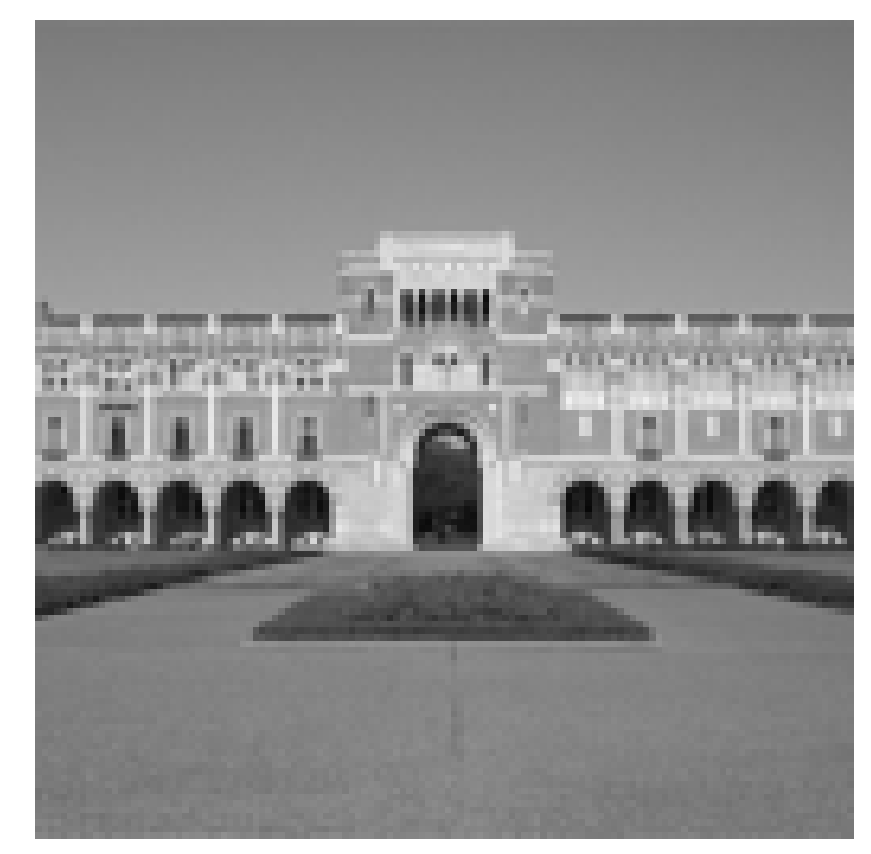
\includegraphics[width=0.24\linewidth]{./fig/lovett_original.pdf} &
		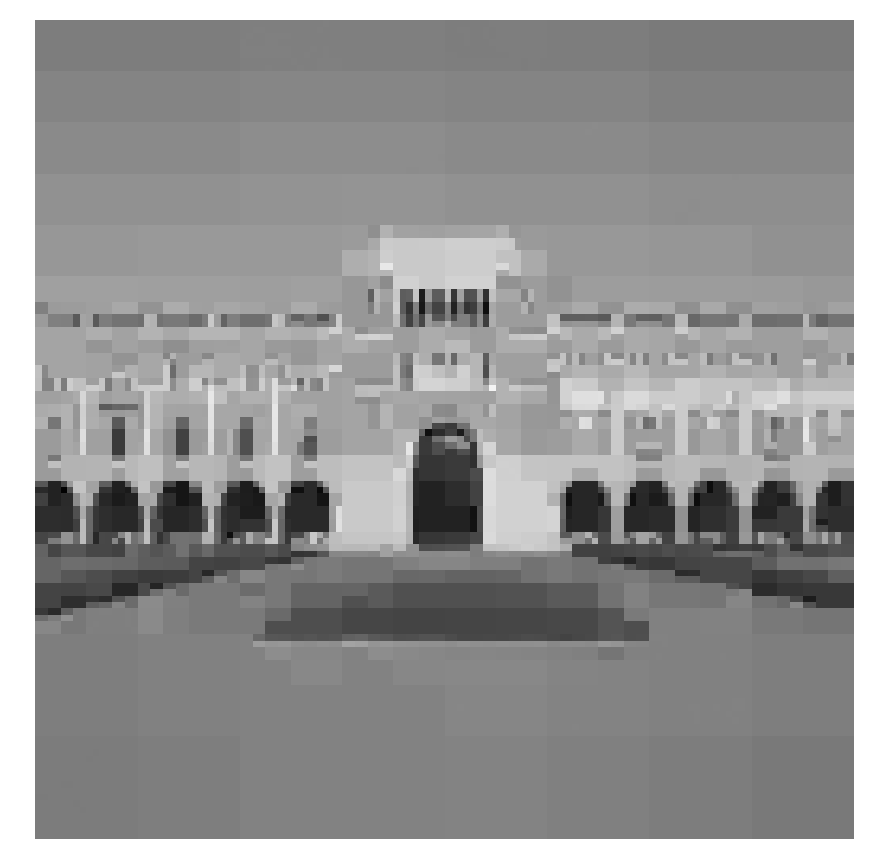
\includegraphics[width=0.24\linewidth]{./fig/lovett_r1.pdf} &
		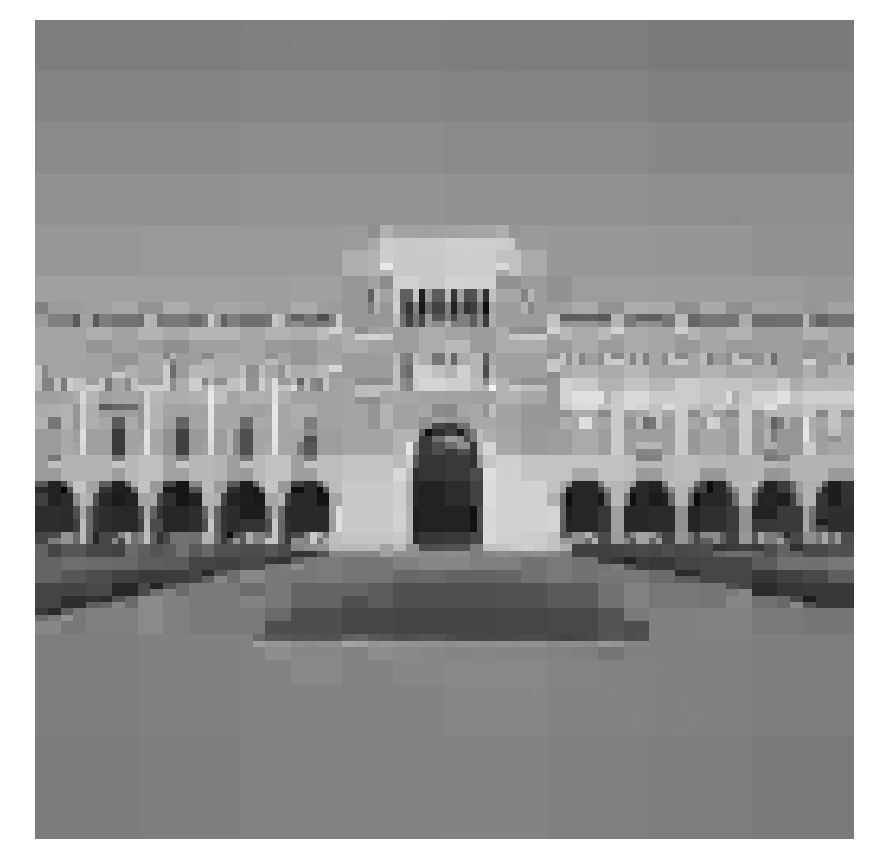
\includegraphics[width=0.24\linewidth]{./fig/lovett_r2.pdf} &
		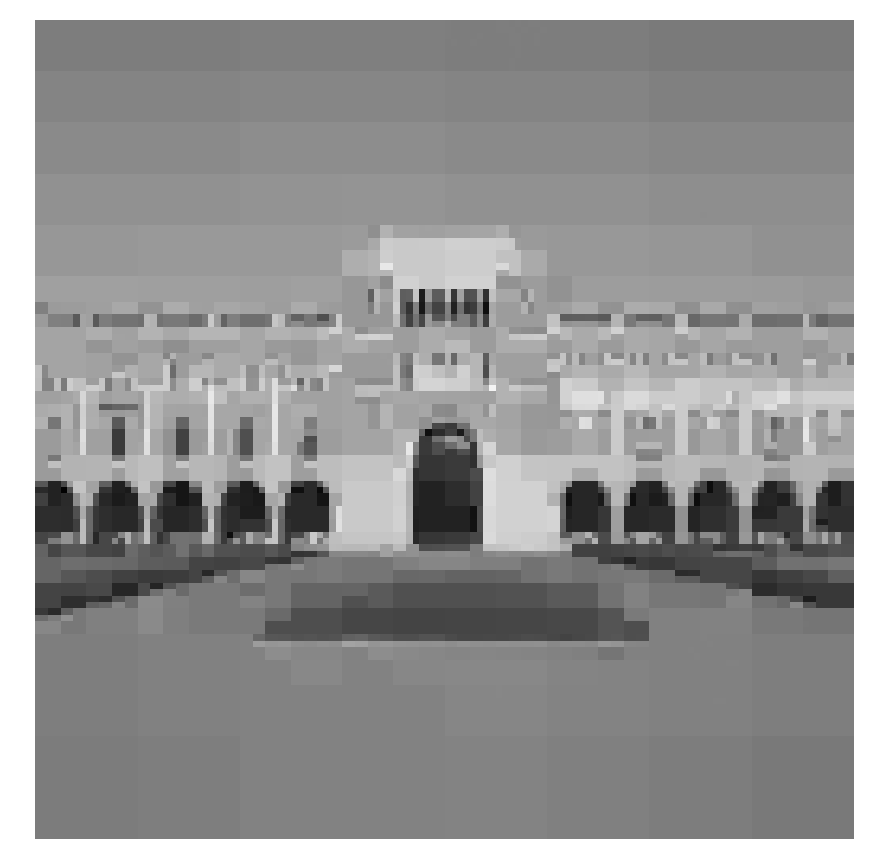
\includegraphics[width=0.24\linewidth]{./fig/lovett_r4.pdf}  \\
		(a) & (b) & (c) & (d)
	\end{tabular}
	\end{center}
	\caption{{(a) Original Lovett Hall image ($n=16,384$); sparse reconstructions ($s=1000$) using $m=8000$ measurements for (b) $R=1$, (c) $R=2$, (d) $R=4$}}
	\label{fig:lovett}
\end{figure*}

%\begin{figure}[h]
%	\begin{center}
%		%\vspace{-0em}
%		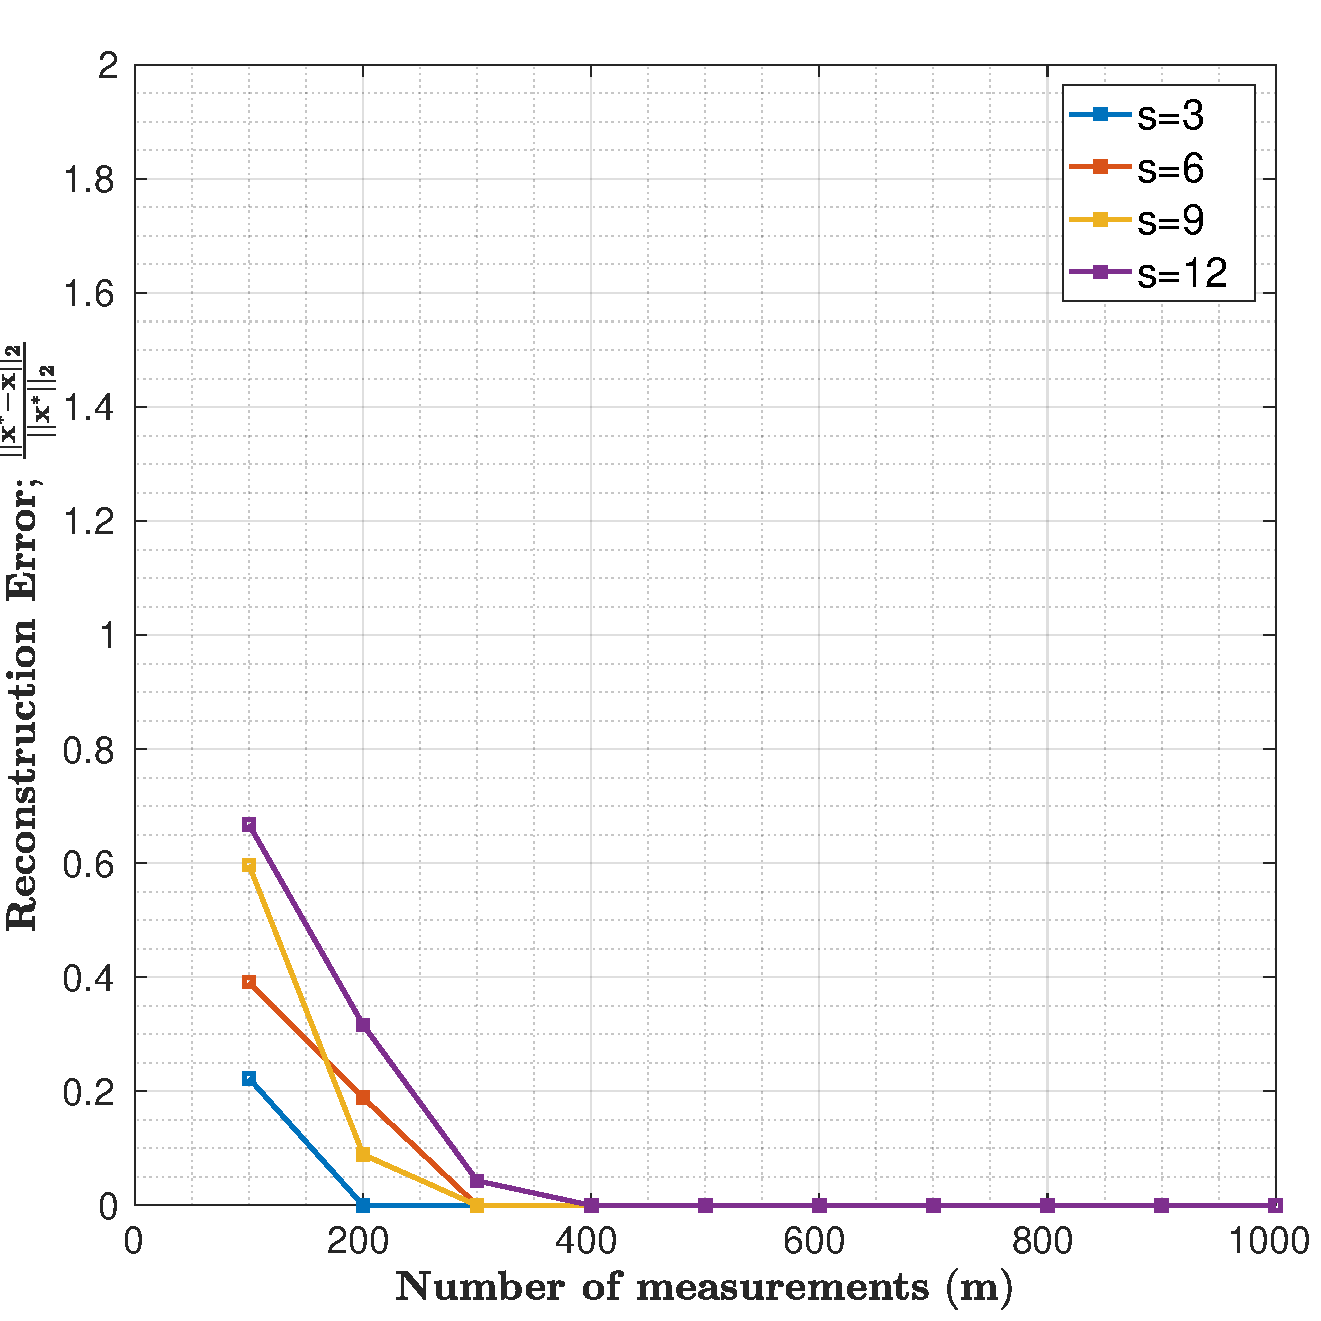
\includegraphics[width=0.9\linewidth]{./fig/rconst_rcm_amp_1_r_1_s_3_12_m_100_1000_justice-pursuit.pdf}
%	\end{center}
%	\caption{{Mean relative reconstruction error vs no. of measurements $(m)$ for MoRAM with $\norm{\mb{x^*}}_2=1,R=1,n=1000$.}}
%	\label{fig:plot-r-1}
%\end{figure}


%\begin{figure}[t]
%	\begin{center}
%		%\vspace{-0em}
%		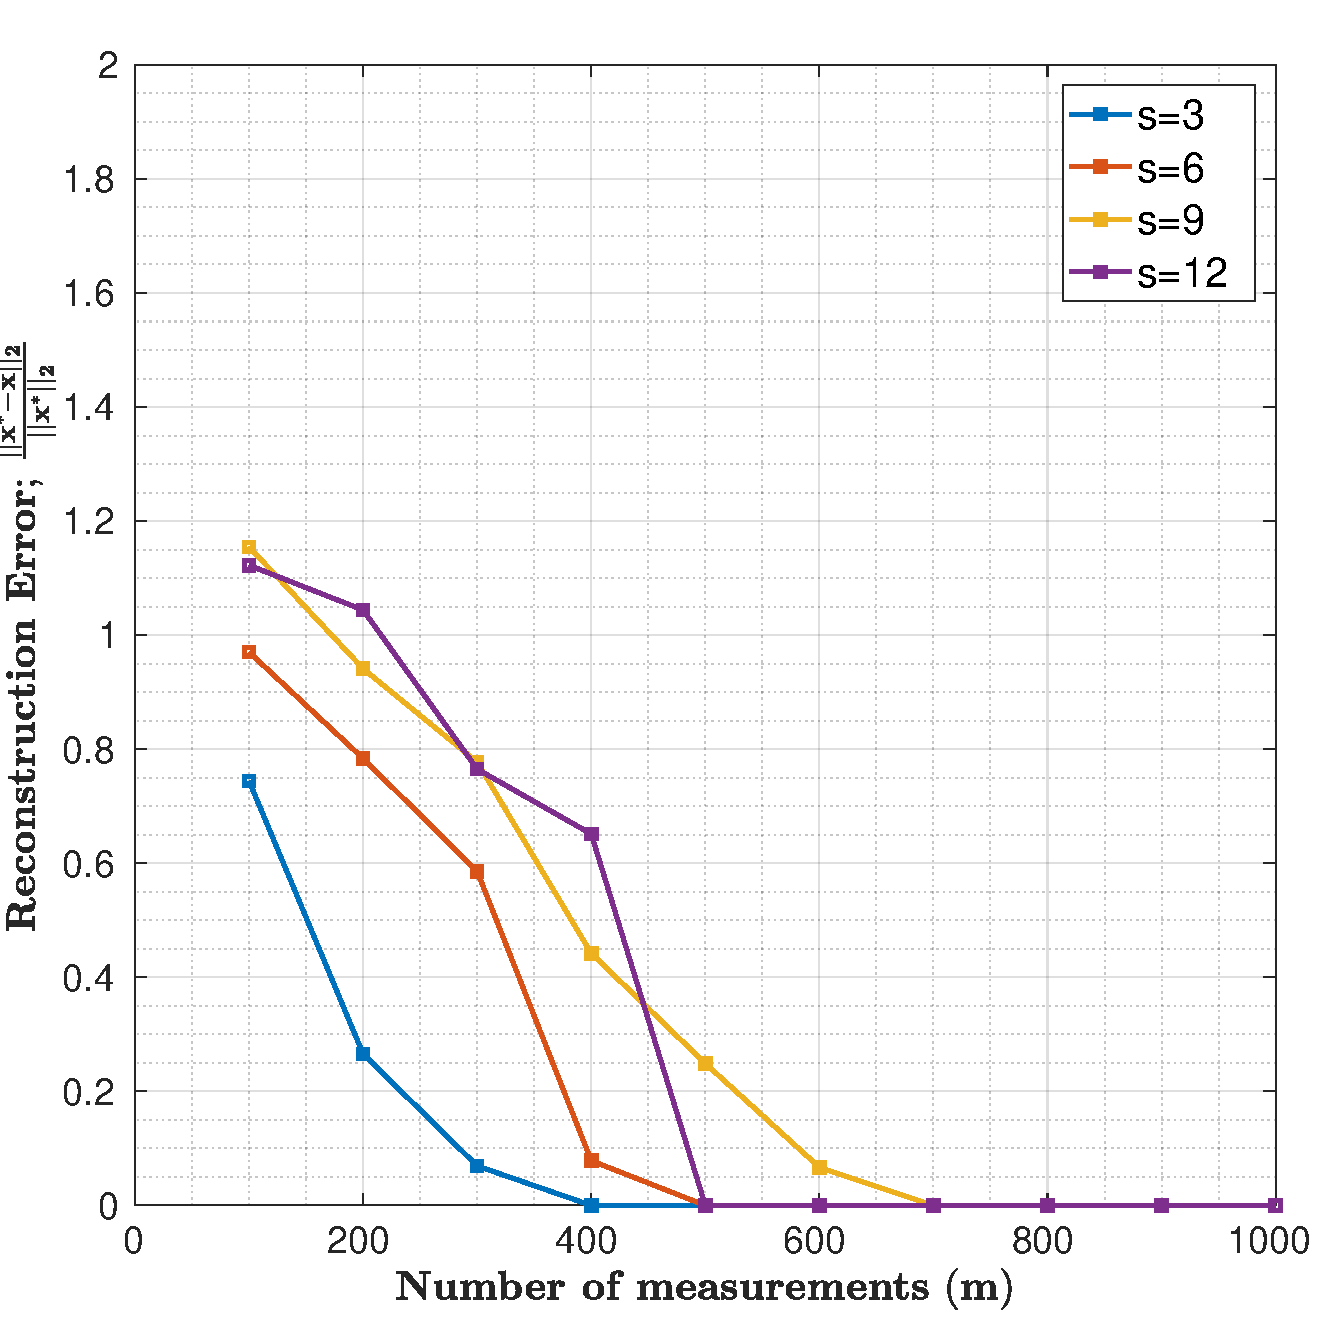
\includegraphics[width=0.9\linewidth]{./fig/rconst_rcm_amp_1_r_2_s_3_12_m_100_1000_justice-pursuit.pdf}
%	\end{center}
%	\caption{{Mean relative reconstruction error vs no. of measurements $(m)$ for MoRAM with $\norm{\mb{x^*}}_2=1,R=2,n=1000$.}}
%	\label{fig:plot-r-2}
%\end{figure}
%
%
%\begin{figure}[t]
%	\begin{center}
%		%\vspace{-0em}
%		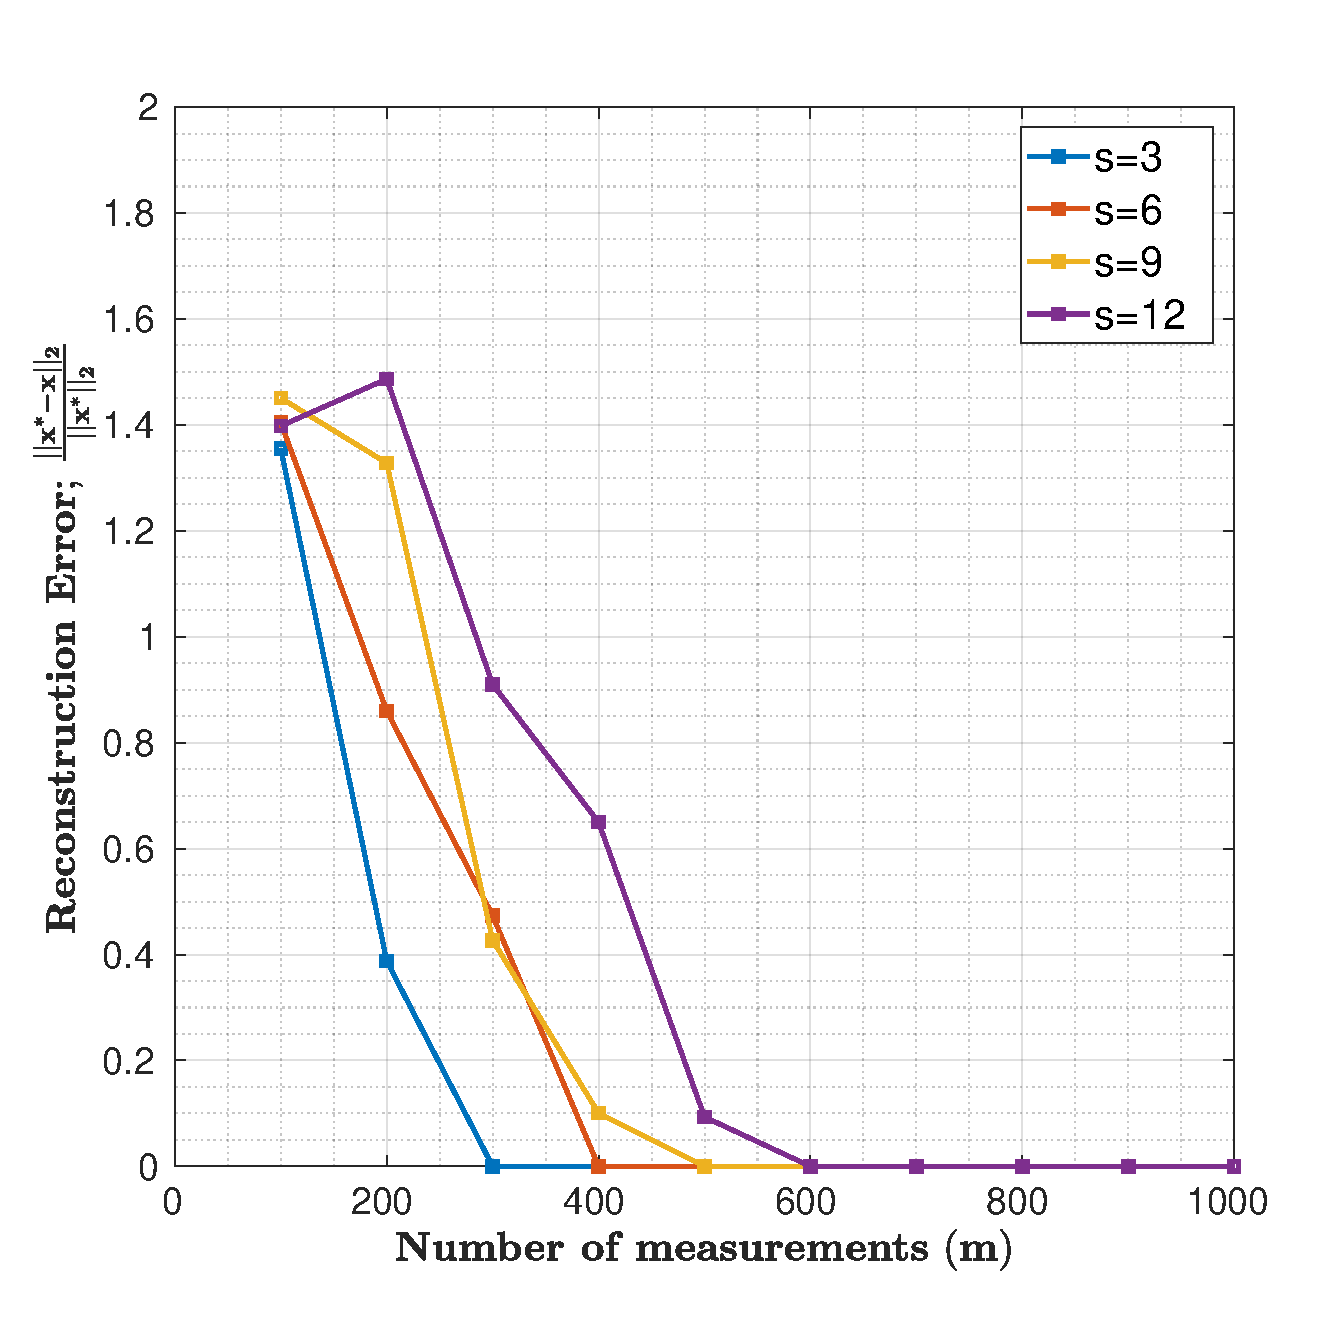
\includegraphics[width=0.9\linewidth]{./fig/rconst_rcm_amp_1_r_4_s_3_12_m_100_1000_justice-pursuit.pdf}
%	\end{center}
%	\caption{{Mean relative reconstruction error vs no. of measurements $(m)$ for MoRAM with $\norm{\mb{x^*}}_2=1,R=4,n=1000$.}}
%	\label{fig:plot-r-4}
%\end{figure}


%\begin{figure}[h]
%	\begin{center}
%		%\vspace{-0em}
%		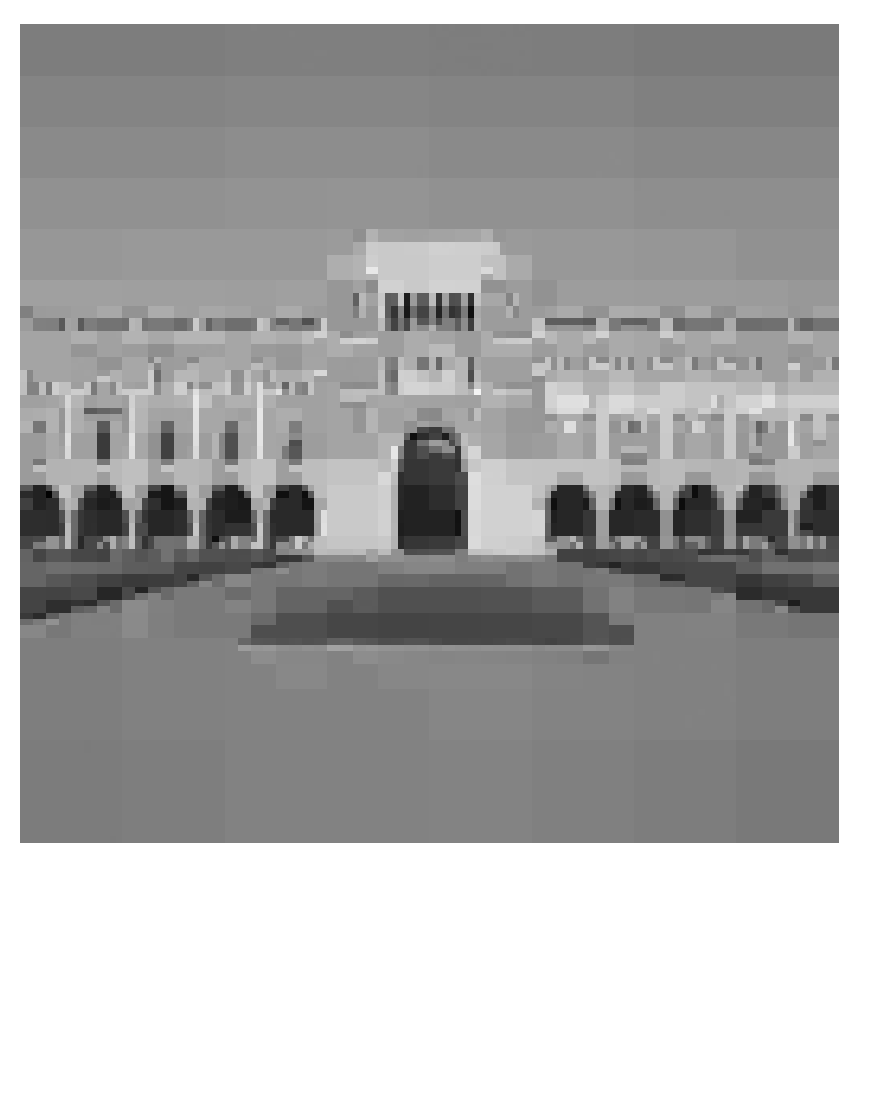
\includegraphics[width=0.9\linewidth]{./fig/reconst_lovett.pdf}
%	\end{center}
%	\caption{{Reconstruction using MoRAM}}
%	\label{fig:lovettreconst}
%\end{figure}
\begin{figure}[!t]
	\centering
	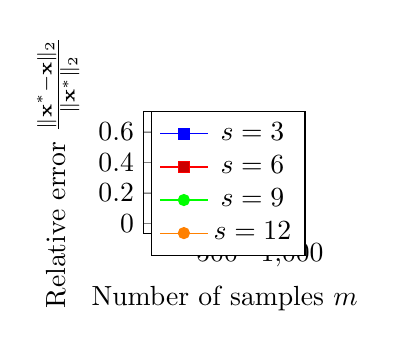
\begin{tikzpicture}
\begin{axis}
[width=0.3\textwidth,
xlabel= Number of samples $m$, 
ylabel= Relative error $\frac{\norm{\mb{x^*-x}}_2}{\norm{\mb{x^*}}_2}$,
grid style = dashed,
grid=both,
legend style=
{
at={(1,1), %for arxiv version
%at={(1.65,0.8),  %for NIPS version
anchor=top},
cells={align=center}, 
%legend columns=-1,
} 
]

\addplot[color=blue,mark=square*] plot coordinates {
	(100, 0.222952795500352)
	(200, 8.25E-05)
	(300, 6.48E-05)
	(400, 6.37E-05)
	(500, 7.91E-05)
 	(600, 6.45E-05)
	(700, 5.51E-05)
	(800, 4.77E-05)
	(900, 6.78E-05)
	(1000, 5.76E-05)
};
\addlegendentry{$s=3$};


\addplot plot coordinates {
(100,	0.391717206388554)
(200,	0.189009904901885)
(300,	8.75E-05)
(400,	6.63E-05)
(500,	7.39E-05)
(600,	6.96E-05)
(700,	5.79E-05)
(800,   6.41E-05)
(900,	8.06E-05)
(1000,	6.78E-05)
};

\addlegendentry{$s=6$};


\addplot[color=green,mark=*] plot coordinates {
(100,0.596874049564358)
(200,0.0893297570309944)
(300,0.0000961819292563893)
(400,0.0000965366166880477)
(500,0.0000950192717929039)
(600,0.0000992956375702069)
(700,0.0000835965044892149)
(800,0.0000675354618845817)
(900,0.0000811820156888768)
(1000,0.000064977150825922)
};
\addlegendentry{$s=9$};

\addplot[color=orange,mark=*] plot coordinates {
(100,0.667881390121055)
(200,0.316701449929789)
(300,0.0432277244535189)
(400,0.000108785027973407)
(500,0.0000962070190416804)
(600,0.0000899199807562489)
(700,0.000102447155819804)
(800,0.0000922462885218879)
(900,0.0000888147784526045)
(1000,0.0000753141220088111)

};
\addlegendentry{$s=12$};



%\legend{CoPRAM\\Block CoPRAM\\ThWF\\SPARTA\\}

\end{axis}
\end{tikzpicture}
	\caption{\sl Mean relative reconstruction error vs no. of measurements $(m)$ for MoRAM with $\norm{\mb{x^*}}_2=1,R=1,n=1000$.} \label{fig:plot-r-1}
\end{figure}

\begin{figure}[!t]
	\centering
	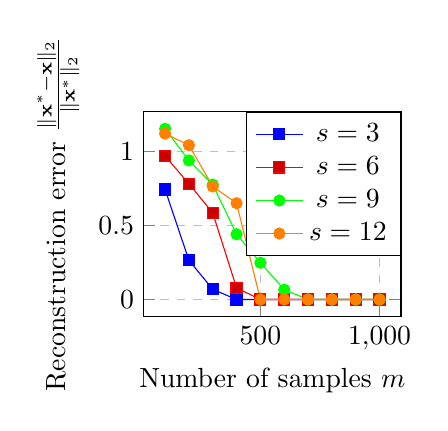
\begin{tikzpicture}
\begin{axis}
[width=0.4\textwidth,
xlabel= Number of samples $m$, 
ylabel= Reconstruction error $\frac{\norm{\mb{x^*-x}}_2}{\norm{\mb{x^*}}_2}$,
grid style = dashed,
grid=both,
legend style=
{
	at={(1,1), %for arxiv version
		%at={(1.65,0.8),  %for NIPS version
		anchor=top},
	cells={align=center}, 
	%legend columns=-1,
} 
]

\addplot[color=blue,mark=square*] plot coordinates {
	(100,0.74427083497336)
	(200,0.26556282505296)
	(300,0.0693282329160152)
	(400,0.0000759947449506268)
	(500,0.0000703837475666469)
	(600,0.0000522047439857151)
	(700,0.0000638145267540324)
	(800,0.000053588062967525)
	(900,0.0000341906002745844)
	(1000,0.0000649790103329161)
	
};
\addlegendentry{$s=3$};


\addplot plot coordinates {
	(100,0.970200248504512)
	(200,0.783733967580109)
	(300,0.585896829880407)
	(400,0.0785807046200051)
	(500,0.0000841836424731131)
	(600,0.0000758879406272977)
	(700,0.0000712248016620914)
	(800,0.0000609478657003822)
	(900,0.0000823001981803784)
	(1000,0.0000652284523240285)
	
};

\addlegendentry{$s=6$};


\addplot[color=green,mark=*] plot coordinates {
	(100,1.15475705568194)
	(200,0.941209335557007)
	(300,0.777520369268922)
	(400,0.442101179084315)
	(500,0.249049460556818)
	(600,0.066874088406845)
	(700,0.0000934401692366995)
	(800,0.0000832753637218933)
	(900,0.0000718321294789104)
	(1000,0.0000674942823198963)
	
};
\addlegendentry{$s=9$};

\addplot[color=orange,mark=*] plot coordinates {
	(100,1.12249994092088)
	(200,1.04403070665004)
	(300,0.76510361311149)
	(400,0.65138560583711)
	(500,0.000087283006450878)
	(600,0.000101093733403955)
	(700,0.0000771972799083333)
	(800,0.0000768498307046639)
	(900,0.0000962856213515402)
	(1000,0.0000790639986588349)
};
\addlegendentry{$s=12$};



%\legend{CoPRAM\\Block CoPRAM\\ThWF\\SPARTA\\}

\end{axis}
\end{tikzpicture}
	\caption{\sl Mean relative reconstruction error vs no. of measurements $(m)$ for MoRAM with $\norm{\mb{x^*}}_2=1,R=2,n=1000$.} \label{fig:plot-r-2}
\end{figure}

\begin{figure}[!t]
	\centering
	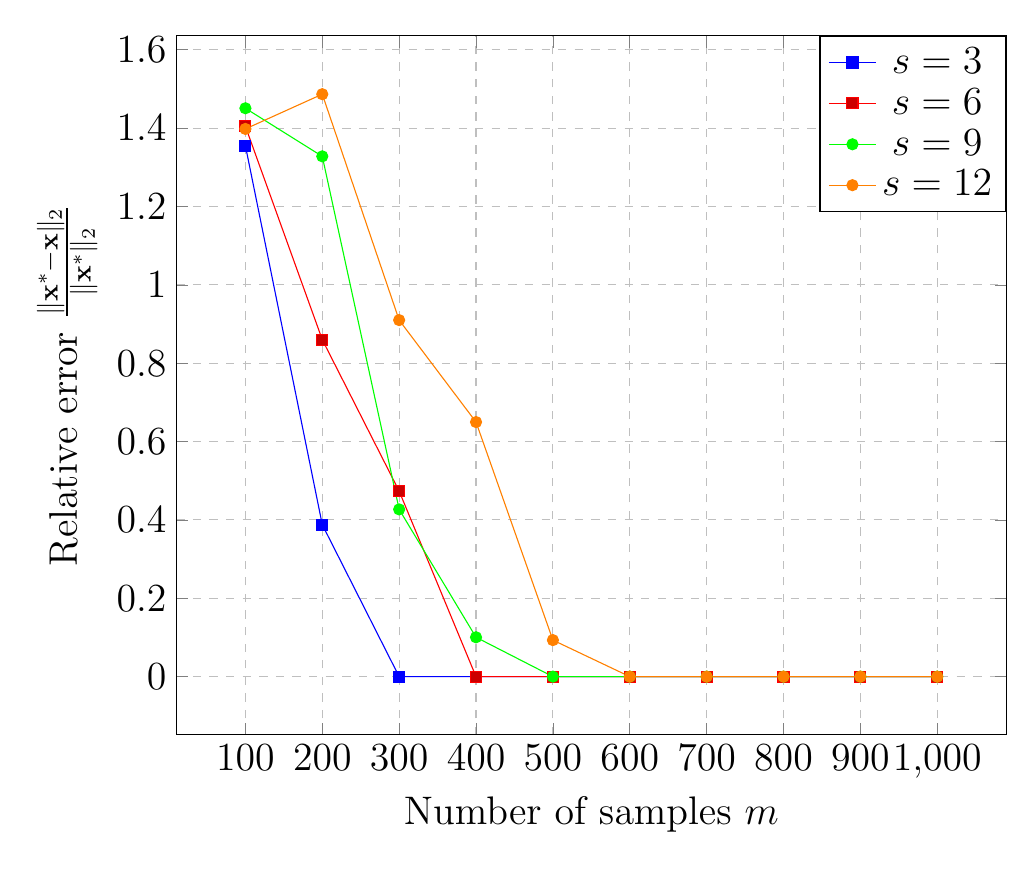
\begin{tikzpicture}
\tikzstyle{every node}=[font=\Large]
\begin{axis}
[width=\linewidth,
xlabel= Number of samples $m$, 
ylabel= Relative error $\frac{\norm{\mb{x^*-x}}_2}{\norm{\mb{x^*}}_2}$,
grid style = dashed,
grid=both,
legend style=
{
at={(1,1), %for arxiv version
%at={(1.65,0.8),  %for NIPS version
anchor=top},
cells={align=center}, 
%legend columns=-1,
} 
]

\addplot[color=blue,mark=square*] plot coordinates {
(100,1.35491249236152)
(200,0.387834861360979)
(300,0.0000838932462760031)
(400,0.0000796709195404289)
(500,0.0000699847485553827)
(600,0.0000654248964096406)
(700,0.0000556622044076941)
(800,0.0000577754338669424)
(900,0.0000476093461140991)
(1000,0.000050430624642886)

};
\addlegendentry{$s=3$};


\addplot plot coordinates {
(100,1.4044226284938)
(200,0.860030446367654)
(300,0.473492899335313)
(400,0.0000833934372627376)
(500,0.0000824008767554939)
(600,0.0000637716674864768)
(700,0.0000644672859553126)
(800,0.0000649831938234799)
(900,0.0000692018122982395)
(1000,0.0000633648746645319)

};

\addlegendentry{$s=6$};


\addplot[color=green,mark=*] plot coordinates {
(100,1.45063072923552)
(200,1.32791017206988)
(300,0.426899433442911)
(400,0.100521404653474)
(500,0.0000847861906819546)
(600,0.0000874052339854557)
(700,0.0000975048393826316)
(800,0.000072296472052776)
(900,0.0000706944130642887)
(1000,0.0000730819848601016)

};
\addlegendentry{$s=9$};

\addplot[color=orange,mark=*] plot coordinates {
(100,1.39786595436235)
(200,1.48655013005159)
(300,0.909955665520478)
(400,0.649802110302209)
(500,0.0932660496014009)
(600,0.0000913091790977068)
(700,0.000104507094662964)
(800,0.0000965628384101342)
(900,0.0000934605996504098)
(1000,0.0000841210242777489)	
};
\addlegendentry{$s=12$};



%\legend{CoPRAM\\Block CoPRAM\\ThWF\\SPARTA\\}

\end{axis}
\end{tikzpicture}
	\caption{\sl Mean relative reconstruction error vs no. of measurements $(m)$ for MoRAM with $\norm{\mb{x^*}}_2=1,R=4,n=1000$.} \label{fig:plot-r-4}
\end{figure}


%	\section{Discussion}
\label{sec:disc}
In this paper, for signal recovery from compressed modulo measurements, we presented a novel algorithmic approach inspired from the classical phase retrieval solutions. Our mathematical and experimental analysis support our claim of exact signal recovery through proposed algorithm. Several open questions remain that can serve as the future directions of our work. While in this paper we considered only two periods within the modulo operation, extending the proposed approach for more periods (and theoretically infinite periods) in a significant and interesting research direction. Instead of relying on sparsity prior for compressed recovery, employing novel set of priors such as GAN priors\cite{bora2017compressed,shah2018solving} or deep image priors \cite{lacoste2017deep} can also be a direction to be explored. Moreover, our analysis is limited to the case of Gaussian measurements, thus extending our results to various measurement schemes such as Fourier samples can be an interesting problem for future study. 
	{{
	\footnotesize
	\bibliographystyle{IEEEbib}
	\bibliography{vsbib}
	}
	}	
\end{document}

